%--------------------------------------------------------------------------
% Dokumentenklasse
%--------------------------------------------------------------------------

% disable Warning for remreset Package
% \RequirePackage{silence}
% \WarningFilter{remreset}{The remreset package}

\documentclass[
	pagesize,
	fontsize=12pt,
	paper=a4,
	oneside,
   reqno
]{scrartcl}

%--------------------------------------------------------------------------
% Standardpakete 
%--------------------------------------------------------------------------
\usepackage[ngerman]{babel}               % Deutsch Silbentrennung
\usepackage[T1]{fontenc}                  % Font Type
\usepackage[utf8]{inputenc}               % Font Encoding
\usepackage{lmodern}                      % Latin Modern Font
\usepackage{csquotes}                     % Setzen von Zitaten
\usepackage{xspace}                       % setzten von Leerzeichen nach Abkürzungen
\usepackage{microtype}                    % für glattere Seitenränder
\renewcommand*\familydefault{\sfdefault}  % Serifen lose Schrift
%\renewcommand*\familydefault{\ttdefault} % Schreibmaschinenschrift

%--------------------------------------------------------------------------
% Extra Packages
%--------------------------------------------------------------------------

% Abkürzungspaket
\usepackage{acronym}

% Symbolverzeichnis
\usepackage[symbols,nogroupskip,nonumberlist,sort=use]{glossaries-extra}

% \makenoidxglossaries

\glsxtrnewsymbol[description={Gewichtskraft}]{FG}{\ensuremath{F_{\mathrm{G}}}}
\glsxtrnewsymbol[description={Gewichtskraft in Bewegungsrichtung}]{FG1}{\ensuremath{F^{'}_{\mathrm{G}}}}
\glsxtrnewsymbol[description={Bewegungskraft des Schlittens}]{Fa}{\ensuremath{F_{\mathrm{a}}}}
\glsxtrnewsymbol[description={Pendelkraft}]{FP}{\ensuremath{F_{\mathrm{P}}}}
\glsxtrnewsymbol[description={Pendelkraft in Bewegungsrichtung}]{FP1}{\ensuremath{F^{'}_{\mathrm{P}}}}
\glsxtrnewsymbol[description={Reibkraft}]{Ff}{\ensuremath{F_{\mathrm{f}}}}
\glsxtrnewsymbol[description={Coulombsche Reibung}]{FC}{\ensuremath{F_{\mathrm{C}}}}
\glsxtrnewsymbol[description={Gesamtkraft}]{Fges}{\ensuremath{F_{\mathrm{ges}}}}
\glsxtrnewsymbol[description={Pendelmoment}]{MP}{\ensuremath{M_{\mathrm{P}}}}
\glsxtrnewsymbol[description={Gewichtsmoment}]{MG}{\ensuremath{M_{\mathrm{G}}}}
\glsxtrnewsymbol[description={Reibmoment}]{Mf}{\ensuremath{M_{\mathrm{f}}}}
\glsxtrnewsymbol[description={Gesamtmoment}]{Mges}{\ensuremath{M_{\mathrm{ges}}}}

% Mathe Pakete
\usepackage{amsmath}
\DeclareMathOperator{\sgn}{sgn}
\usepackage{thmtools}
\usepackage{amsfonts}
\usepackage{amssymb}
\usepackage{mathtools}
\usepackage{breqn}
\usepackage{empheq}

% Listenumgebungen
\usepackage{listings}
\usepackage{paralist}
\usepackage{enumitem}
\usepackage{adjustbox}

% Demo Text
\usepackage{blindtext}

% Farb-Pakete
\usepackage{xcolor}
\usepackage{fancyvrb}
\usepackage{colortbl}

% Farbedefinitionen
\definecolor{htw}{RGB}{120, 184, 2}
\definecolor{ccW}{RGB}{255,255,255}
\definecolor{ccR}{RGB}{197,14,31}
\definecolor{ccG}{RGB}{113,113,113}
\definecolor{ccL}{RGB}{220,220,220}
\definecolor{ccS}{RGB}{0,0,0}
\definecolor{ccB}{RGB}{68,73,159}
\definecolor{ccD}{RGB}{0,0,80}
\definecolor{grey}{RGB}{200,200,200}
\definecolor{lightGrey}{RGB}{230,230,230}

% Für erweiterte Tabellen
\usepackage{longtable}
\usepackage{tabularx}
\usepackage{float}
\usepackage{multirow}
\usepackage{makecell}
% \setlength{\tabcolsep}{0.5em}       % for the horizontal padding
% {\renewcommand{\arraystretch}{1.8}  % for the vertical padding
% \usepackage{ragged2e}
% \newcolumntype{R}[1]{>{\RaggedRight}p{#1}}

% Einheitenpaket
\usepackage[exponent-product = \cdot]{siunitx}
\sisetup{locale=DE}
\sisetup{parse-numbers = false}

\makeatletter
\renewcommand\@dotsep{5}
\makeatother

% Pakete für Grafiken
\usepackage{graphicx}
\usepackage{wrapfig}
\usepackage{overpic}
\usepackage{epstopdf}
\usepackage{caption}
\usepackage{subcaption}
\usepackage{rotating}
\usepackage{lscape}
% \captionsetup[subfigure]{list=true, font=normalsize, labelformat=brace, position=top} %setup für subfigure captions

% Diagramm-/Grafikerstellung
\usepackage{pstricks}
\usepackage{tikz}
\usetikzlibrary{patterns,patterns.meta}
\makeatletter
\pgfkeys{/pgf/.cd,
  parallelepiped offset x/.initial=2mm,
  parallelepiped offset y/.initial=2mm
}
\pgfdeclareshape{parallelepiped}
{
  \inheritsavedanchors[from=rectangle] % this is nearly a rectangle
  \inheritanchorborder[from=rectangle]
  \inheritanchor[from=rectangle]{north}
  \inheritanchor[from=rectangle]{north west}
  \inheritanchor[from=rectangle]{north east}
  \inheritanchor[from=rectangle]{center}
  \inheritanchor[from=rectangle]{west}
  \inheritanchor[from=rectangle]{east}
  \inheritanchor[from=rectangle]{mid}
  \inheritanchor[from=rectangle]{mid west}
  \inheritanchor[from=rectangle]{mid east}
  \inheritanchor[from=rectangle]{base}
  \inheritanchor[from=rectangle]{base west}
  \inheritanchor[from=rectangle]{base east}
  \inheritanchor[from=rectangle]{south}
  \inheritanchor[from=rectangle]{south west}
  \inheritanchor[from=rectangle]{south east}
  \backgroundpath{
    % store lower right in xa/ya and upper right in xb/yb
    \southwest \pgf@xa=\pgf@x \pgf@ya=\pgf@y
    \northeast \pgf@xb=\pgf@x \pgf@yb=\pgf@y
    \pgfmathsetlength\pgfutil@tempdima{\pgfkeysvalueof{/pgf/parallelepiped offset x}}
    \pgfmathsetlength\pgfutil@tempdimb{\pgfkeysvalueof{/pgf/parallelepiped offset y}}
    \def\ppd@offset{\pgfpoint{\pgfutil@tempdima}{\pgfutil@tempdimb}}
    \pgfpathmoveto{\pgfqpoint{\pgf@xa}{\pgf@ya}}
    \pgfpathlineto{\pgfqpoint{\pgf@xb}{\pgf@ya}}
    \pgfpathlineto{\pgfqpoint{\pgf@xb}{\pgf@yb}}
    \pgfpathlineto{\pgfqpoint{\pgf@xa}{\pgf@yb}}
    \pgfpathclose
    \pgfpathmoveto{\pgfqpoint{\pgf@xb}{\pgf@ya}}
    \pgfpathlineto{\pgfpointadd{\pgfpoint{\pgf@xb}{\pgf@ya}}{\ppd@offset}}
    \pgfpathlineto{\pgfpointadd{\pgfpoint{\pgf@xb}{\pgf@yb}}{\ppd@offset}}
    \pgfpathlineto{\pgfpointadd{\pgfpoint{\pgf@xa}{\pgf@yb}}{\ppd@offset}}
    \pgfpathlineto{\pgfqpoint{\pgf@xa}{\pgf@yb}}
    \pgfpathmoveto{\pgfqpoint{\pgf@xb}{\pgf@yb}}
    \pgfpathlineto{\pgfpointadd{\pgfpoint{\pgf@xb}{\pgf@yb}}{\ppd@offset}}
  }
}
\makeatother
\usetikzlibrary{math}
\usepackage{pgfplots}
\pgfplotsset{compat=1.5}
\usetikzlibrary{intersections,positioning,arrows,automata,calc,patterns,shapes.multipart,fit,backgrounds,decorations.pathreplacing}
\usetikzlibrary{decorations,shapes.geometric}
\usetikzlibrary{matrix,calc,angles,positioning,quotes}
% \usepackage{tikz-uml}

\usepackage{pgfkeys}
\usepackage{pgfopts}
\usepackage{ifthen}
\usepackage{xstring}
\usepackage{calc}
\usepackage{pst-plot,pst-bar,pst-node} % Balkendiagramme
\usepackage{capt-of}
\usepackage{incgraph} % Fullscreen Images
\usepackage{pdfpages} % Include external pdf pages

\usepackage{latexsym}
\usepackage{censor}
\usepackage{here}
% \StopCensoring        % Auskommentiert wird der Text entschwaerzt 
% \censor{Oszilloskop}  % Befehl zum einschwärzen
\usepackage{trfsigns}   % Transformation Symbol o---o \laplace and \Laplace
\usepackage{circuitikz}

\usepackage{multido}

% Verlinkungen im Text
\usepackage{url}
\usepackage{hyperref}
\PassOptionsToPackage{hyphens}{url}
\hypersetup{hidelinks}
\urlstyle{same}

%--------------------------------------------------------------------------
% Eigene Befehle
%--------------------------------------------------------------------------
\newcommand*\widefbox[1]{\fbox{\hspace{1em}#1\hspace{1em}}} % Box für align-Umgebung

%------------sectioning command-------------------
% The sectioning command one level down the hierarchy from \subsubsection is called \paragraph followed by \subparagraph
% to include this in your table of contents

% Tiefe des Inhaltsverzeichnis
\setcounter{tocdepth}{2}
\setcounter{secnumdepth}{4}

% Abkürzungen durch Kommandos setzen
\newcommand{\bspw}{bspw.\xspace}
\newcommand{\bzw}{bzw.\xspace}
\newcommand{\etc}{etc.\xspace}
\newcommand{\zB}{z.\,B.\xspace}
\newcommand{\EV}{e.\,V.\xspace}
\newcommand{\zT}{z.\,T.\xspace}
\newcommand{\iVm}{i.\,V.\,m.\xspace}
\newcommand{\idR}{i.\,d.\,R.\xspace}
\newcommand{\ihv}{i.\,H.\,v.\xspace}
\newcommand{\ua}{u.\,a.\xspace}
\newcommand{\dH}{d.\,h.\xspace}
\newcommand{\vgl}{vgl.\xspace}
\newcommand{\ca}{ca.\xspace}
\newcommand{\dV}{d.\,Verf.}
\newcommand{\RNr}{Rn.\xspace}
\newcommand{\oa}{o.\,{ä}.\xspace}
\newcommand{\vC}{v.\,Chr.\xspace}
\newcommand{\nC}{n.\,Chr.\xspace}
\newcommand{\vA}{v.\,a.\xspace}
\newcommand{\eng}{engl.\xspace}
\newcommand{\tabitem}{~~\llap{\textbullet}~~}

%------------Zitate-------------------------------
\newcommand*{\zitat}[2]{%
   \normalfont\small
   \begin{quote}
   \glqq#1\grqq \par
   #2
   \end{quote}
   \normalsize
}
\newcommand*{\zitatmitueberschrift}[3]{%
   \normalfont\small
   \begin{quote} #3
   \glqq#1\grqq \par
   #2
   \end{quote}
   \normalsize
}
\newcommand*{\zitext}[2]{%
   \glqq#1\grqq\ %
   [#2]%
}

%-----------Seitendesign--------------------------
\usepackage[width=15.5cm, height=23cm, includeheadfoot]{geometry}
\geometry{paper=a4paper}
% \usepackage[left=6cm,right=1cm,top=1.5cm, bottom=1cm, includeheadfoot]{geometry}
% \newgeometry{oneside}
% \setlength{\voffset}{0cm}
\setlength{\headheight}{1.1\baselineskip} % increase headheight
\setlength{\footheight}{28.99998pt}       % increase foodheight
\setlength{\parindent}{0cm}               % Einrücken nach \newline
\setlength{\footskip}{86pt}               % Move Footer down
% \setlength{\topmargin}{0cm}
% \setlength{\marginparsep}{0.5cm}
% \setlength{\marginparwidth}{1.5cm}
% \setlength{\textwidth}{16cm}
% \setlength{\textheight}{23cm}
% \setlength{\oddsidemargin}{1cm}
% \setlength{\evensidemargin}{2cm}

%----------Kopf & Fußzeile------------------------
% \usepackage[headsepline,footsepline]{scrpage2}
\usepackage[headsepline]{scrlayer-scrpage}
\pagestyle{scrheadings}
\clearpairofpagestyles
\ihead{\headmark}
\automark{section}
\chead{}
\ohead{
\includegraphics[scale=0.09]{Bilder/HTWLogoKopfzeile.png} \nocite{HTWklein}}
\ifoot{Richter, Zielstorff\\ Laarsen, Schmiedehausen}
\cfoot{\pagemark}
\ofoot{M2 Modellbildung/\\ Simulation}

%--------------------------------------------------------------------------
% Beginn des Dokuments
%--------------------------------------------------------------------------
\begin{document}

%----------Deckblatt----------------------------- 
\begin{titlepage}
   \pagestyle{empty} % setzt Pagestyle-Befehl

   % HTW Logo
   \begin{flushright}
   
\includegraphics[scale=.07]{Bilder/LogoHTWBerlin.png}  \nocite{HTWgross}
   \end{flushright}

   \vspace{1cm}

   % Titel
   \begin{center}
      \Huge{\textbf{Schwungrad Pendel: Modellbildung/Simulation (M2)}} \\
   \end{center}

   \vspace{3cm}

   % Name
   \begin{flushleft}
      \begin{tabular}{l c l }
         \textbf{Name: }&\hspace{1 cm} &\textbf{Matrikelnummer:} \\
         Milan Laarsen          & & 581929 \\
         Sebastian Richter      & & 572906 \\
         Cyrill Schmiedehausen  & & XXXXXX \\
         Aaron Zielstorff       & & 567183 \\
      \end{tabular}
   \end{flushleft}

   \vspace{1cm}

   % Daten
   \begin{tabular}{l l}
      \textbf{Fachbereich:}   & FB1                                                     \\
      \textbf{Studiengang:}   & M.\xspace Elektrotechnik                                \\
      \textbf{Fachsemester:}  & 2.\xspace FS                                            \\
      \textbf{Fach:}          & M2 Modellbildung/Simulation                             \\
      \textbf{Dozent:}        & Prof.\xspace Dr.\xspace -Ing.\xspace Steffen Borchers   \\
      \textbf{Abgabe am:}     & 26.\xspace August 2022                                  \\ 
   \end{tabular}
\end{titlepage}
\clearpage

%--------Inhaltsverzeichnis-----------------------
\renewcommand{\contentsname}{Inhaltsverzeichnis}
\tableofcontents
\clearpage

%--------Abbildungsverzeichnis--------------------
\renewcommand{\listfigurename}{Abbildungsverzeichnis}
\renewcommand*{\figurename}{Abb.}
\listoffigures
% \clearpage

%--------Tabellenverzeichnis----------------------
\renewcommand*{\listtablename}{Tabellenverzeichnis}
\renewcommand*{\tablename}{Tab.}
\listoftables
\clearpage

%----------Symbolverzeichnis----------------------
% \printnoidxglossary[type=symbols,style=long,title={Symbolverzeichnis}]
% \clearpage

%---------Kapitel/Text----------------------------

%\pagestyle{aaron}
\section{Einführung und Versuchsaufbau} \label{sec:Einfuehrung}

Inhalt dieser Belegarbeit ist die Modellierung eines inversen Pendels, welches über ein Schwungrad regelungstechnisch in der aufrechten Position stabil gehalten werden soll.\\
Diese Arbeit geht dabei im ersten Abschnitt auf den \textbf{Versuchsaufbau} und die \textbf{Modellierung} des Pendels ein. Es schließt sich eine \textbf{Sensitivitäts- und Parameteranalyse} an, über welche der Einfluss bestimmter Modellgrößen auf das Verhalten des Systems untersucht wird. \\
Nachdem das Modell aufgestellt und auf seine Eigenschaften analysiert wurde, folgt die Implementierung als Simulation in Matlab/Simulink. Dafür soll zunächst das \textbf{Aufschwingen des Pendels}. umgesetzt werden. Kann das Pendel bis in einen bestimmten Bereich um die obere Ruhelage bewegt werden, übernimmt ein \textbf{einfacher Zustandsregler}, welcher ebenfalls in dieser Arbeit entworfen wird. \\
Abschließend wird ein \textbf{Beobachter} umgesetzt, über welchen die nicht messbaren Zustände des Systems rekonstruiert werden können, um den Regler am realen Versuch in Betrieb zu nehmen.

Nachfolgend findet sich die Darstellung der Modellparameter/Konstanten zur Modellierung des Schwungrad-Pendels (siehe \autoref{tab:Tabelle1.1}).

\begin{table}[H]
    \centering
    \begin{tabular}{|lll|}
        \hline
        \rowcolor{grey}
        \textbf{Symbol}     & \textbf{Parameter}                                & \textbf{Wert/Einheit}                         \\ \hline
        $\theta$            & Winkel des Pendels                                & $\SI{}{rad}$                                  \\
        $\varphi$           & Winkel des Schwungrades                           & $\SI{}{rad}$                                  \\
        $J_{\mathrm{1}}$    & Trägheitsmoment des Pendels (+ Motorstator)       & $\SI{0.01186}{kg \cdot m^2}$                  \\
        $J_{\mathrm{2}}$    & Trägheitsmoment des Rads (+ Motorrotor)           & $\SI{0.0005711}{kg \cdot m^2}$                \\
        $c_{\mathrm{1}}$    & Reibungsfaktor des Pendels                        & $\SI{0.04}{\frac{N \cdot m \cdot s}{rad}}$    \\
        $c_{\mathrm{2}}$    & Reibungsfaktor des Rads                           & $\SI{0.0001}{\frac{N \cdot m \cdot s}{rad}}$  \\
        $m_{\mathrm{1}}$    & Masse des Pendels und Stators                     & $\SI{0.826}{kg}$                              \\
        $m_{\mathrm{2}}$    & Masse des Rads und Rotors                         & $\SI{0.583}{kg}$                              \\
        $l_{\mathrm{1}}$    & Länge vom Ursprung bis Schwerpunkt des Pendels    & $\SI{0.1053}{m}$                              \\
        $l_{\mathrm{2}}$    & Länge vom Ursprung bis Schwerpunkt des Rads       & $\SI{0.14}{m}$                                \\
        $K_{\mathrm{b}}$    & Back-End-Konstante                                & $\SI{0.0987}{\frac{V}{\frac{rad}{s}}}$        \\
        $K_{\mathrm{t}}$    & Motor-Drehmoment-Konstante                        & $\SI{0.0987}{\frac{N \cdot m}{A}}$            \\
        $R_{\mathrm{a}}$    & Widerstand der Ankerwicklung                      & $\SI{1.5562}{\Omega}$                         \\ \hline
    \end{tabular}
    \caption{Modellparameter des Schwungrad-Pendels}
    \label{tab:Tabelle1.1}
\end{table}

Ziel der Arbeit soll es sein, anhand von Beispielparametern eine effektive Regelung umzusetzen, welche später bei der Übernahme auf einen realen Versuchsaufbau einfach adaptiert werden kann. Dazu ist es wichtig ein gutes Modell umzusetzen und den Einfluss der verschiedenen Modell- und Regelparameter auf das Verhalten des Systems zu kennen.\\

\autoref{fig:Bild1.1} zeigt den modellhaften Versuchsaufbau. Das System besteht aus einem Pendel und einem Schwungrad. Das Pendel kann frei rotieren um die 0z-Achse, die senkrecht zur 0xy-Ebene steht. Das Schwungrad wird durch einen Gleichstrommotor angetrieben und dreht sich um eine Achse parallel zur 0z-Achse. Das Pendel kann durch die Reaktionskraft ausbalanciert werden, die durch das Schwungrad erzeugt wird.

\begin{figure}[H]
   \centering
   \fbox{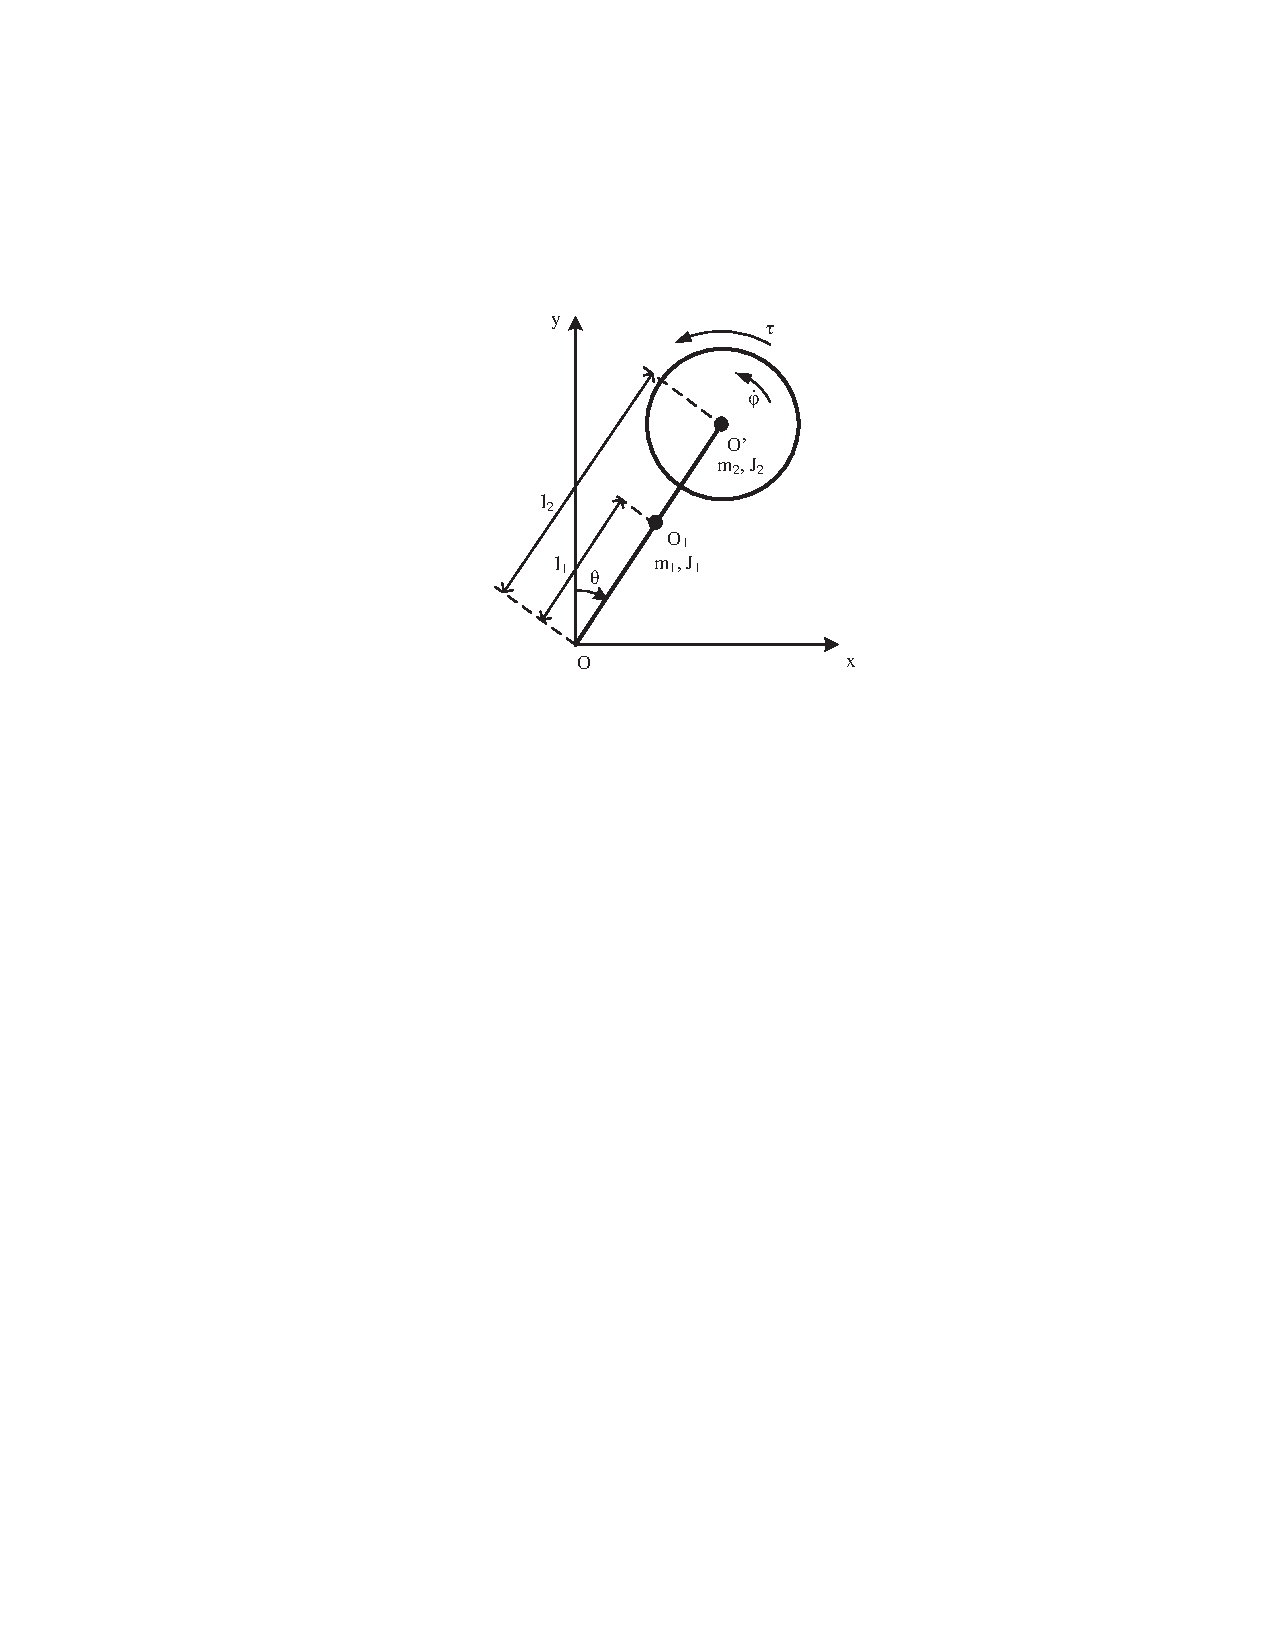
\includegraphics[width=0.4\textwidth]{Bilder/1. einfuehrung/Versuchsaufbau.pdf}}
   \caption[Modellskizze des Versuchs]{Modellskizze des Schwungrad-Pendel-Versuchs inklusive relevanter Modellparameter}
   \label{fig:Bild1.1}
\end{figure}

Weiterhin gelten folgende Voraussetzungen für das System:

\begin{itemize}
    \item Das Pendel ist frei gelagert.
    \item Der Motor (Gleichstrommaschine) ist spannungsgeregelt (bei $V_{\mathrm{m,Max}} = \SI{20}{V}$).
    \item Der Winkel ($\theta$) des Pendels und der Winkel ($\varphi$) des Schwungrades werden gemessen.
\end{itemize}

Es sind folgende Einschränkungen ermittelt/festgelegt worden:

\begin{itemize}
    \item Das Aufschwingen soll über eine schnelle Steuerung umgesetzt werden.
    \item Es soll ein Zustandsregler mit vier Zuständen ($x_{\mathrm{1}}$ bis $x_{\mathrm{4}}$) verwendet werden für die Regelung um die Ruhelage.
    \item Für die Ermittlung der Winkelgeschwindigkeiten ($\dot\theta$ und $\dot\varphi$) ist die Rekonstruktion über einen Beobachter notwendig.
\end{itemize}

%\pagestyle{aaron}
\section{Modellierung des Schwungrad-Pendels} \label{sec:Modellierung}

Der folgende Abschnitt beschäftigt sich mit der Modellierung des Schwungrad-Pendels inklusive des treibenden Gleichstrommotors.

\subsection{Modellierung des Gleichstrommotors}

\begin{figure}[H]
    \centering
    \fbox{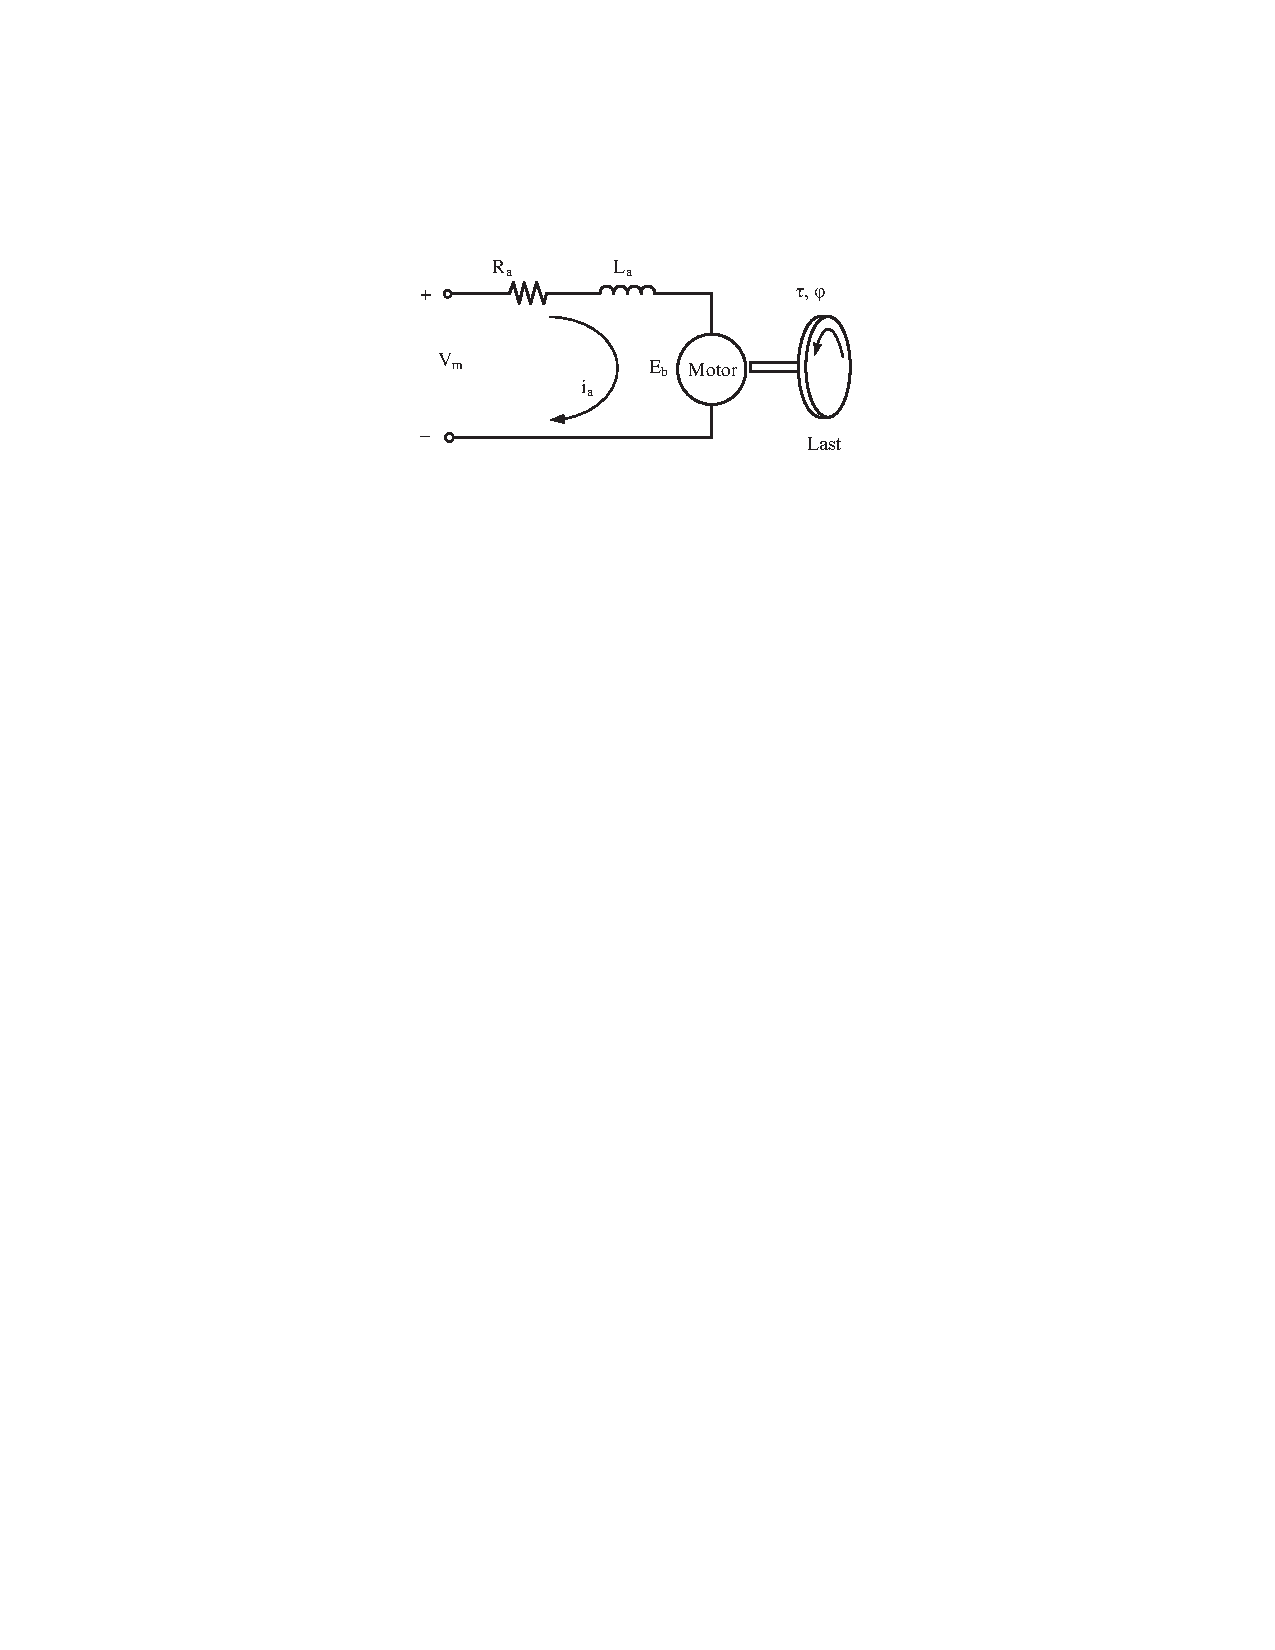
\includegraphics[width=0.6\textwidth]{Bilder/2_modellierung/Ersatzschaltbild.pdf}}
    \caption[Ersatzschaltbild Gleichstrommotor]{Ersatzschaltbild des Gleichstrommotors am Schwungrad-Pendel}
    \label{fig:Bild2.1}
\end{figure}

\autoref{fig:Bild2.1} zeigt das Ersatzschaltbild des Gleichstrommotors am Schwungrad-Pendel. Das zweite Kirchhoff'sche Gesetzt ergibt folgende Gleichung:

\begin{equation} \label{eq:Gleichung2.1}
    V_{\mathrm{m}} = i_{\mathrm{a}} R_{\mathrm{a}} + L_{\mathrm{a}} \frac{di_{\mathrm{a}}}{dt} + E_{\mathrm{b}}
\end{equation}
\newline
Die gegenelektromotorische Kraft (EMK) hängt von der Winkelgeschwindigkeit $\dot\varphi$ und der Gegen-EMK-Konstante $K_{\mathrm{b}}$ wie folgt ab:

\begin{equation} \label{eq:Gleichung2.2}
    E_{\mathrm{b}} = K_{\mathrm{b}} \dot\varphi
\end{equation}
\newline
Angenommen die Wirkung der Induktivität ist sehr klein ($L_{\mathrm{a}} \ll R_{\mathrm{a}}$), \autoref{eq:Gleichung2.1} ergibt sich zu

\begin{equation} \label{eq:Gleichung2.3}
    i_{\mathrm{a}} = \frac{V_{\mathrm{m}} - K_{\mathrm{b}} \dot\varphi}{R_{\mathrm{a}}}.
\end{equation}
\newline
Das Motordremoment $\tau$ ist mit dem Ankerstrom $i_{\mathrm{a}}$ durch eine Motordrehmomentkonstante $K_{\mathrm{t}}$ verbunden. Die Modellgleichung des Gleichstrommotors ergibt sich somit zu:

\begin{equation} \label{eq:Gleichung2.4}
    \boxed{\tau = K_{\mathrm{t}} i_{\mathrm{a}} = K_{\mathrm{t}} \frac{V_{\mathrm{m}} - K_{\mathrm{b}} \dot\varphi}{R_{\mathrm{a}}}}
\end{equation}

\subsection{Modellierung des Schwungrad-Pendels}

Zur Modellierung des Pendels wurde der Langrange-Ansatz gewählt, um die Bewegungsgleichungen des Pendels herzuleiten.
 
\subsubsection{Lagrange Ansatz}

Die nachfolgende Gleichung zeigt den \textbf{Lagrange Ansatz} unter Berücksichtigung der \textbf{dissipativen Funktion}. Diese besagt in Erweiterung zu der Lagrange-Formulierung, dass Energie in einem Vorgang in Wärme umgewandelt wird. Mit Hilfe der dissipativen Funktion können \textbf{Reibungsverluste} bei der Energiemethode nach Lagrange berücksichtigt werden.
\begin{equation} \label{eq:Gleichung2.5}
    \boxed{\frac{d}{dt} \left(\frac{\partial L}{\partial \dot{q_{\mathrm{i}}}}\right) - \frac{\partial L}{\partial q_{\mathrm{i}}} + \frac{\partial D}{\partial \dot{q_{\mathrm{i}}}} = 0}
\end{equation}

\subsubsection{Freiheitsgrade und Zwangsbedingungen}

In \autoref{fig:Bild1.1} sind zwei Teilchen \bzw Massepunkte im $\mathbb{R}^2$ zu erkennen. Zum Einen die des Pendels und zum Anderen die des Schwungrades. Somit gilt grundsätzlich:

\begin{itemize}
    \item 2 Punkte: 4 Freiheitsgrade (FHG)
\end{itemize}

Das Schwungrad-Pendel besitzt jedoch auch zwei Zwangsbedingungen, die wie folgt formuliert werden können:

\begin{itemize}
    \item Das Pendel kann nur um die 0z-Achse rotieren: \\ $z = 0$
    \item Die Masse $m_2$ ist über des Pendel mit dem Aufhängepunkt 0 gekoppelt: \\ $(y_{\mathrm{m_1}} - y_{\mathrm{m_2}})^2 + (x_{\mathrm{m_1}} - x_{\mathrm{m_2}})^2 = l_2^2$
\end{itemize}

Beide Zwangsbedingungen sind holonom-skleronom, da sie als Gleichungen zwischen zwei Koordinaten angegeben werden können und nicht von der Zeit abhängig sind.

Somit bleiben am Ende noch zwei Freiheitsgrade (FHG) übrig.

\subsubsection{Generalisierte Koordinaten}

Aus den verbliebenen Freiheitsgraden werden die generalisierten Koordinaten abgeleitet. Dabei gilt grundsätzlich folgender Zusammenhang im $\mathbb{R}^2$:

\begin{equation} \label{eq:Gleichung2.6}
    \boxed{S = 2n - k}
\end{equation}
\newline
mit $S$ als Anzahl der Freiheitsgrade und somit auch der Anzahl der generalisierten Koordinaten, $n$ der Anzahl der Teilchen und $k$ der Anzahl der holonomen Zwangsbedingungen.\\
Die beiden Generalisierten Koordinaten sind somit:

\begin{itemize}
    \item $q_{\mathrm{1}} = \theta$
    \item $q_{\mathrm{2}} = \varphi$
\end{itemize}

\subsubsection{Berechnung der kinetischen und potentiellen Energie}

Für die Lagrange-Formulierung werden die kinetische und die potentielle Energie des Systems benötigt. Die kinetische Energie setzt sich zusammen aus der translatorischen kinetischen Energie $E_{\mathrm{kin,trans}}$ und der rotatorischen kinetischen Energie $E_{\mathrm{kin,rot}}$. Die Gleichungen sind nachfolgend aufgestellt.

\begin{align} \label{eq:Gleichung2.7}
    \begin{split}
        E_{\mathrm{kin,trans}} &= \frac{1}{2} m_1 (l_1\dot\theta)^2 + \frac{1}{2}m_2 (l_2\dot\theta)^2 \\
        E_{\mathrm{kin,rot}} &= \frac{1}{2} J_1 (\dot\theta)^2 + \frac{1}{2} J_2 (\dot\theta + \dot\varphi)^2
    \end{split}
\end{align}
\newline
Die gesamte \textbf{kinetische Energie des Systems} ist somit:

\begin{empheq}[box=\widefbox]{align} \label{eq:Gleichung2.8}
    \begin{split}
        E_{\mathrm{kin}} &= E_{\mathrm{kin,trans}} + E_{\mathrm{kin,rot}} \\
        E_{\mathrm{kin}} &= \frac{1}{2} \left( m_1 l_1^2 + m_2 l_2^2 + J_1 + J_2 \right) \dot\theta^2 + J_2\dot\theta\dot\varphi + \frac{1}{2} J_2 \dot\varphi^2
    \end{split}
\end{empheq}
\newline
Der Ursprung der potentiellen Energie liegt bei Null. Somit ergibt sich die \textbf{potentielle Energie des Systems} zu:

\begin{equation} \label{eq:Gleichung2.9}
    \boxed{E_{\mathrm{pot}} = \left( m_1 l_1 + m_2 l_2 \right) g\cos (\theta)}
\end{equation}

\subsubsection{Herleitung der Bewegungsgleichungen}

Die \textbf{Lagrange-Funktion} $L$ wird aus der Differenz der kinetischen Energie aus \autoref{eq:Gleichung2.8} und der potentiellen Energie aus \autoref{eq:Gleichung2.9} berechnet.

\begin{empheq}[box=\widefbox]{align} \label{eq:Gleichung2.10}
    \begin{split}
        L &= E_{\mathrm{kin}} - E_{\mathrm{pot}} \\
        L &= \frac{1}{2} \left( m_1 l_1^2 + m_2 l_2^2 + J_1 + J_2 \right) \dot\theta^2 + J_2\dot\theta\dot\varphi + \frac{1}{2} J_2 \dot\varphi^2 - \left( m_1 l_1 + m_2 l_2 \right) g\cos (\theta)
    \end{split}
\end{empheq}
\newline
Die \textbf{dissipative Energie} $D$ ist:

\begin{equation} \label{eq:Gleichung2.11}
    \boxed{D = \frac{1}{2} c_1 \dot\theta^2 + \frac{1}{2} c_2 \dot\varphi^2}
\end{equation}
\newline
Zieht man nun den Ansatz aus \autoref{eq:Gleichung2.5} heran und wendet diesen für die generalisierte Koordinate $\theta$ an, so erhält man die \textbf{Bewegungsgleichung des Schwungrades}:

\begin{equation} \label{eq:Gleichung2.12}
    \boxed{\left( m_1 l_1^2 + m_2 l_2^2 + J_1 + J_2\right) \ddot\theta + J_2\ddot\varphi + c_1\dot\theta - \left( m_1 l_1 + m_2 l_2 \right) g\sin (\theta) = 0}
\end{equation}
\newline
Ebenfalls der Gleiche Ansatz wird nun für die generalisierte Koordinate $\varphi$ angewendet:

\begin{equation} \label{eq:Gleichung2.13}
    J_2 \left( \ddot\theta + \ddot\varphi \right) + c_2 \dot\varphi = \tau
\end{equation}
\newline
Setzt man nun \autoref{eq:Gleichung2.4} in \autoref{eq:Gleichung2.13} ein erhält man die \textbf{Bewegungsgleichung des Pendels}:

\begin{equation} \label{eq:Gleichung2.14}
    \boxed{J_2 \left( \ddot\theta + \ddot\varphi \right) + c_2 \dot\varphi = K_{\mathrm{t}} i_{\mathrm{a}} = K_{\mathrm{t}} \frac{V_{\mathrm{m}} - K_{\mathrm{b}} \dot\varphi}{R_{\mathrm{a}}}}
\end{equation}

%\pagestyle{aaron}
\section{Zustandsraumdarstellung} \label{sec:Zustandsraumdarstellung}

Um das Verhalten mittels mathematischer Beziehungen zu veranschaulichen, wird die \textbf{Zustandsraumdarstellung} verwendet. Der \textbf{Systemeingang} wird festgelegt mit

\begin{equation} \label{eq:Gleichung3.1}
    \underline{u} = V_{\mathrm{m}},
\end{equation}
\newline
wobei $V_{\mathrm{m}}$ die Eingangsspannung des Gleichstrommotors aus \autoref{eq:Gleichung2.1} ist.Die \textbf{Systemzustände} des Schwungrad-Pendels sind:

\begin{align}
    \underline{x} &=
    \begin{bmatrix} \label{eq:Gleichung3.2}
        x_{\mathrm{1}} \\
        x_{\mathrm{2}} \\
        x_{\mathrm{3}} \\
        x_{\mathrm{4}}
    \end{bmatrix} =
    \begin{bmatrix}
        \varphi     \\
        \dot\varphi \\
        \theta      \\
        \dot\theta
    \end{bmatrix}
\end{align}
\newline
Nach zeitlicher Ableitung des Zustandsvektors ergibt sich der \textbf{Vektor der Zustandsänderung} zu:

\begin{align}
    \underline{x} &=
    \begin{bmatrix} \label{eq:Gleichung3.3}
        \dot x_{\mathrm{1}} \\
        \dot x_{\mathrm{2}} \\
        \dot x_{\mathrm{3}} \\
        \dot x_{\mathrm{4}}
    \end{bmatrix} =
    \begin{bmatrix}
        \dot\varphi     \\
        \ddot\varphi    \\
        \dot\theta      \\
        \ddot\theta
    \end{bmatrix}
\end{align}
\newline
Die \textbf{Ausgänge des Systems} gleichen den den vier Zuständen und ergeben sich somit zu

\begin{align}
    \underline{y} &=
    \begin{bmatrix} \label{eq:Gleichung3.4}
        \varphi     \\
        \dot\varphi \\
        \theta      \\
        \dot\theta
    \end{bmatrix}.
\end{align}

\subsection{Nichtlineares Zustandsraummodell}\label{cap:nichtlinearesZustandsraummodell}

Zum Aufstellen des nichtlinearen Zustandsraummodells werden die \autoref{eq:Gleichung2.12} und \autoref{eq:Gleichung2.14} nach den höchsten Ableitungen von $\ddot\varphi$ und $\ddot\theta$ umgestellt.

\begin{align} \label{eq:Gleichung3.5}
    \begin{split}
        \ddot\varphi &= \frac{K_{\mathrm{t}} \frac{V_{\mathrm{m}} - K_{\mathrm{b}} \dot\varphi}{R_{\mathrm{a}}} - c_2 \dot\varphi - J_2 \cdot \ddot\theta}{J_2} \\
        \ddot\theta &= \frac{-J_2 \ddot\varphi - c_1 \dot\theta + \left( m_1 l_1 + m_2 l_2\right) g \sin(\theta)}{m_1 l_1^2 + m_2 l_2^2 + J_1 + J_2}
    \end{split}
\end{align}
\newline
Beide Gleichungen sind über die die Winkelbeschleunigung des Schwungrades $\ddot\varphi$ und die des Pendels $\ddot\theta$ miteinander verkoppelt. Durch das gegenseitige ineinander Einsetzen werden die Abhängigkeiten eliminiert.

\begin{align} \label{eq:Gleichung3.6}
    \begin{split}
        \ddot\varphi &= \frac{K_{\mathrm{t}} \frac{V_{\mathrm{m}} - K_{\mathrm{b}} \dot\varphi}{R_{\mathrm{a}}} - c_2 \dot\varphi - J_2 \cdot \left( \frac{-J_2 \ddot\varphi - c_1 \dot\theta + \left( m_1 l_1 + m_2 l_2\right) g \sin(\theta)}{m_1 l_1^2 + m_2 l_2^2 + J_1 + J_2}\right)}{J_2} \\
        \ddot\theta &= \frac{-J_2 \left( \frac{K_{\mathrm{t}} \frac{V_{\mathrm{m}} - K_{\mathrm{b}} \dot\varphi}{R_{\mathrm{a}}} - c_2 \dot\varphi - J_2 \cdot \ddot\theta}{J_2}\right) - c_1 \dot\theta + \left( m_1 l_1 + m_2 l_2\right) g \sin(\theta)}{m_1 l_1^2 + m_2 l_2^2 + J_1 + J_2}
    \end{split}
\end{align}
\newline
Mit Hilfe der Gleichungen \ref{eq:Gleichung3.1}, \ref{eq:Gleichung3.2} und \ref{eq:Gleichung3.3}, durch das einsetzen in \autoref{eq:Gleichung3.6} und dem Zusammenfassen und Umstellen nach $\ddot\varphi$ \bzw $\ddot\theta$ folgt das \textbf{nichtlineare Zustandsraummodell}.

\begin{empheq}[box=\widefbox]{align} \label{eq:Gleichung3.7}
    \underline{\dot x} =
    \begin{bmatrix}
        x_{\mathrm{2}} \\
        \frac{\frac{K_{\mathrm{t}} \cdot \frac{V_{\mathrm{m}} - K_{\mathrm{b}} \cdot x_4}{R_{\mathrm{a}}} - c_2 \cdot x_4 - \left( m_1 l_1 + m_2 l_2\right) g\sin(x_1) + c_1 \cdot x_2}{J_2}}{1 - \frac{m_1 l_1^2 + m_2 l_2^2 + J_1 + J_2}{J_2}} \\
        x_{\mathrm{4}} \\
        \frac{\frac{\left( m_1 l_1 + m_2 l_2\right) g\sin(x_1) - c_1 \cdot x_2 - \left( m_1 l_1^2 + m_2 l_2^2 + J_1 + J_2\right) \cdot \frac{K_{\mathrm{t}} \cdot \frac{V_{\mathrm{m}} - K_{\mathrm{b}} \cdot x_4}{R_{\mathrm{a}}}}{J_2}}{J_2}}{1 - \frac{m_1 l_1^2 + m_2 l_2^2 + J_1 + J_2}{J_2}}
    \end{bmatrix}
\end{empheq}

\subsection{Lineares Zustandsraummodell}

Das Verhalten des nichtlinearen Systems ist für große Änderungen des Eingangssignals nicht vorhersehbar. Um dennoch Aussagen über das Systemverhalten treffen zu können, wird das nichtlineare Zustandsraummodell mithilfe der Taylorreihenentwicklung um eine Ruhelage ($\underline{x}^{*}$) linearisiert. Die nichtlinearen Restglieder $\underline{R}(\Delta{\underline{x}^2}, \Delta{\underline{u}^2})$ werden zu Null angenommen. Durch die Linearisierung wird das Systemverhalten für kleine Änderungen um die Ruhelage kontrollierbar. Nachfolgend ist die Taylorreihenentwicklung für Linearisierung aufgeführt:

\begin{align} \label{eq:Gleichung3.8}
    \begin{split}
        \dot{\underline{x}}^{*}+\Delta{\dot{\underline{x}}} &=\underline{f}(\underline{x}^{*}+\Delta{\underline{x}},\underline{u}^{*}+\Delta{\underline{u}}) \\
        &=\underline{f}(\underline{x}^{*},\underline{u}^{*})+\left[\frac{\partial f_{\mathrm{i}}}{\partial x_{\mathrm{j}}}\right]_{(\underline{x}^{*}, \underline{u}^{*})}\cdot\Delta{\underline{x}}+\left[\frac{\partial f_{\mathrm{i}}}{\partial u_{\mathrm{j}}}\right]_{(\underline{x}^{*},\underline{u}^{*})}\cdot\Delta{\underline{u}}+\underline{R}(\Delta{\underline{x}^2}, \Delta{\underline{u}^2})
    \end{split}
\end{align}
\newline
Durch die Annahme über das Verhalten der nichtlinearen Restglieder folgt die Struktur des linearen Zustandsraummodells dargestellt in \autoref{eq:Gleichung3.9}.

\begin{align} \label{eq:Gleichung3.9}
    \begin{split}
        \Delta\dot{\underline{x}} &= \left[\frac{\partial f_{\mathrm{i}}}{\partial x_{\mathrm{j}}}\right]_{(\underline{x}^{*}, \underline{u}^{*})}\cdot\Delta{\underline{x}}+\left[\frac{\partial f_{\mathrm{i}}}{\partial u_{\mathrm{j}}}\right]_{(\underline{x}^{*},\underline{u}^{*})}\cdot\Delta{\underline{u}} \\   
        \Delta{\underline{y}} &= \left[\frac{\partial h_{\mathrm{i}}}{\partial x_{\mathrm{j}}}\right]_{(\underline{x}^{*}, \underline{u}^{*})}\cdot\Delta{\underline{x}}+\left[\frac{\partial h_{\mathrm{i}}}{\partial u_{\mathrm{j}}}\right]_{(\underline{x}^{*},\underline{u}^{*})}\cdot\Delta{\underline{u}}
    \end{split}
\end{align}
\newline
Um das linearisierte Zustandsraummodell zu erhalten, werden die einzelnen Gleichungen des nichtlinearen Zustandsraummodells aus \autoref{eq:Gleichung3.7} nach den Zuständen $x_{\mathrm{1}}$ bis $x_{\mathrm{4}}$, sowie dem Eingang $V_{\mathrm{m}}$ partiell abgeleitet und die Ruhelage $\underline{x}^{*}$ eingesetzt. Dabei werden sowohl die Ruhelage des hängenden Pendels (untere Ruhelage) und die des stehenden Pendels (obere Ruhelage) betrachtet. In \autoref{eq:Gleichung3.10} dargestellt ist die untere Ruhelage, mit Hilfe derer das lineare Zustandsraummodell für das hängende Pendel bestimmt werden kann. Anhand dessen kann das lineare Zustandsraummodell in Simulink mit dem nichtlinearen Zustandsraummodell im nachfolgenden Abschnitt (\autoref{sec:Vergleich}) verglichen werden.

\begin{align}\label{eq:Gleichung3.10}
    \begin{split}
        \underline{x}_{\mathrm{1}}^{*}=
        \begin{bmatrix}
            x_{\mathrm{1}}^{*} \\
            x_{\mathrm{2}}^{*} \\
            x_{\mathrm{3}}^{*} \\
            x_{\mathrm{4}}^{*}
        \end{bmatrix}=
        \begin{bmatrix}
            \pi \\
            0   \\
            0   \\
            0
        \end{bmatrix}
    \end{split}
\end{align}
\newline
Die Regelung, welche in \autoref{sec:Zustandsregler} entworfen wird soll dafür sorgen, dass das Pendel in der oberen Ruhelage verweilt. Diese wird beschrieben durch:

\begin{align}\label{eq:Gleichung3.11}
    \begin{split}
        \underline{x}_{\mathrm{2}}^{*}=
        \begin{bmatrix}
            x_{\mathrm{1}}^{*} \\
            x_{\mathrm{2}}^{*} \\
            x_{\mathrm{3}}^{*} \\
            x_{\mathrm{4}}^{*}
        \end{bmatrix}=
        \begin{bmatrix}
            0 \\
            0 \\
            0 \\
            0
        \end{bmatrix}
    \end{split}
\end{align}
\newline
Die allgemeine Form des \textbf{linearen Zustandsraummodells} lautet:

\begin{empheq}[box=\widefbox]{align} \label{eq:Gleichung3.12}
    \begin{split}
        \dot{\underline{x}} &= \underline{A}\cdot\underline{x}+\underline{B}\cdot\underline{u} \\
        \underline{y} &= \underline{C}\cdot\underline{x}+\underline{D}\cdot\underline{u}
    \end{split}
\end{empheq}
\newline
Wendet man nun die Linearisierungsvorschrift aus \autoref{eq:Gleichung3.9} unter Nutzung der Ruhelagen an, so erhält man das konkrete linearisierte Zustandsraummodell für das System. In \autoref{eq:Gleichung3.13} ist das linearisierte Zustandsraummodell für die obere Ruhelage und in \autoref{eq:Gleichung3.14} das für die untere Ruhelage dargestellt.

\begin{empheq}[box=\widefbox]{align} \label{eq:Gleichung3.13}
    \begin{split}
        \Delta{\dot{\underline{x}}}&=
        \begin{bmatrix}
            0           & 1         & 0 & 0         \\
            -50.9760    & -1.2328   & 0 & 0.1960    \\
            0           & 0         & 0 & 1         \\
            50.9760     & 1.2328    & 0 & -11.3323
        \end{bmatrix}\cdot\Delta\underline{x}+
        \begin{bmatrix}
            0       \\
            -1.9548 \\
            0       \\
            113.0101
        \end{bmatrix}\cdot V_{\mathrm{m}}
        \\
        \Delta{\underline{y}} &=
        \begin{bmatrix}
            1 & 0 & 0 & 0 \\
            0 & 0 & 1 & 0
        \end{bmatrix}\cdot\Delta\underline{x}+\underline{0}\cdot V_{\mathrm{m}}
    \end{split}
\end{empheq}

\begin{empheq}[box=\widefbox]{align} \label{eq:Gleichung3.14}
    \begin{split}
        \Delta{\dot{\underline{x}}}&=
        \begin{bmatrix}
            0           & 1         & 0 & 0         \\
            50.9760     & -1.2328   & 0 & 0.1960    \\
            0           & 0         & 0 & 1         \\
            -50.9760    & 1.2328    & 0 & -11.3323
        \end{bmatrix}\cdot\Delta\underline{x}+
        \begin{bmatrix}
            0       \\
            -1.9548 \\
            0       \\
            113.0101
        \end{bmatrix}\cdot V_{\mathrm{m}}
        \\
        \Delta{\underline{y}} &=
        \begin{bmatrix}
            1 & 0 & 0 & 0 \\
            0 & 0 & 1 & 0
        \end{bmatrix}\cdot\Delta\underline{x}+\underline{0}\cdot V_{\mathrm{m}}
    \end{split}
\end{empheq}

%\pagestyle{aaron}
\section{Vergleich lineares/nichtlineares System} \label{sec:Vergleich}

In \autoref{fig:Bild4.1} ist die Übersicht der notwendigen Simulationsstruktur dargestellt. Aus der Übersicht geht hervor, dass beide Systeme unterschiedliche Eingänge besitzen und somit ein direkter Vergleich ohne entsprechende Berücksichtigung der Linearisierungsvorschriften unmöglich ist. Das linearisierte Modell verwendet als Eingang im Gegensatz zum nichtlinearen Modell eine Differenz $\Delta u$. Die Strukturen des nichtlinearen und des linearen Modells sind zur Information in \autoref{fig:Bild4.2} und \autoref{fig:Bild4.3} visualisiert.

\begin{figure}[H]
   \centering
   \fbox{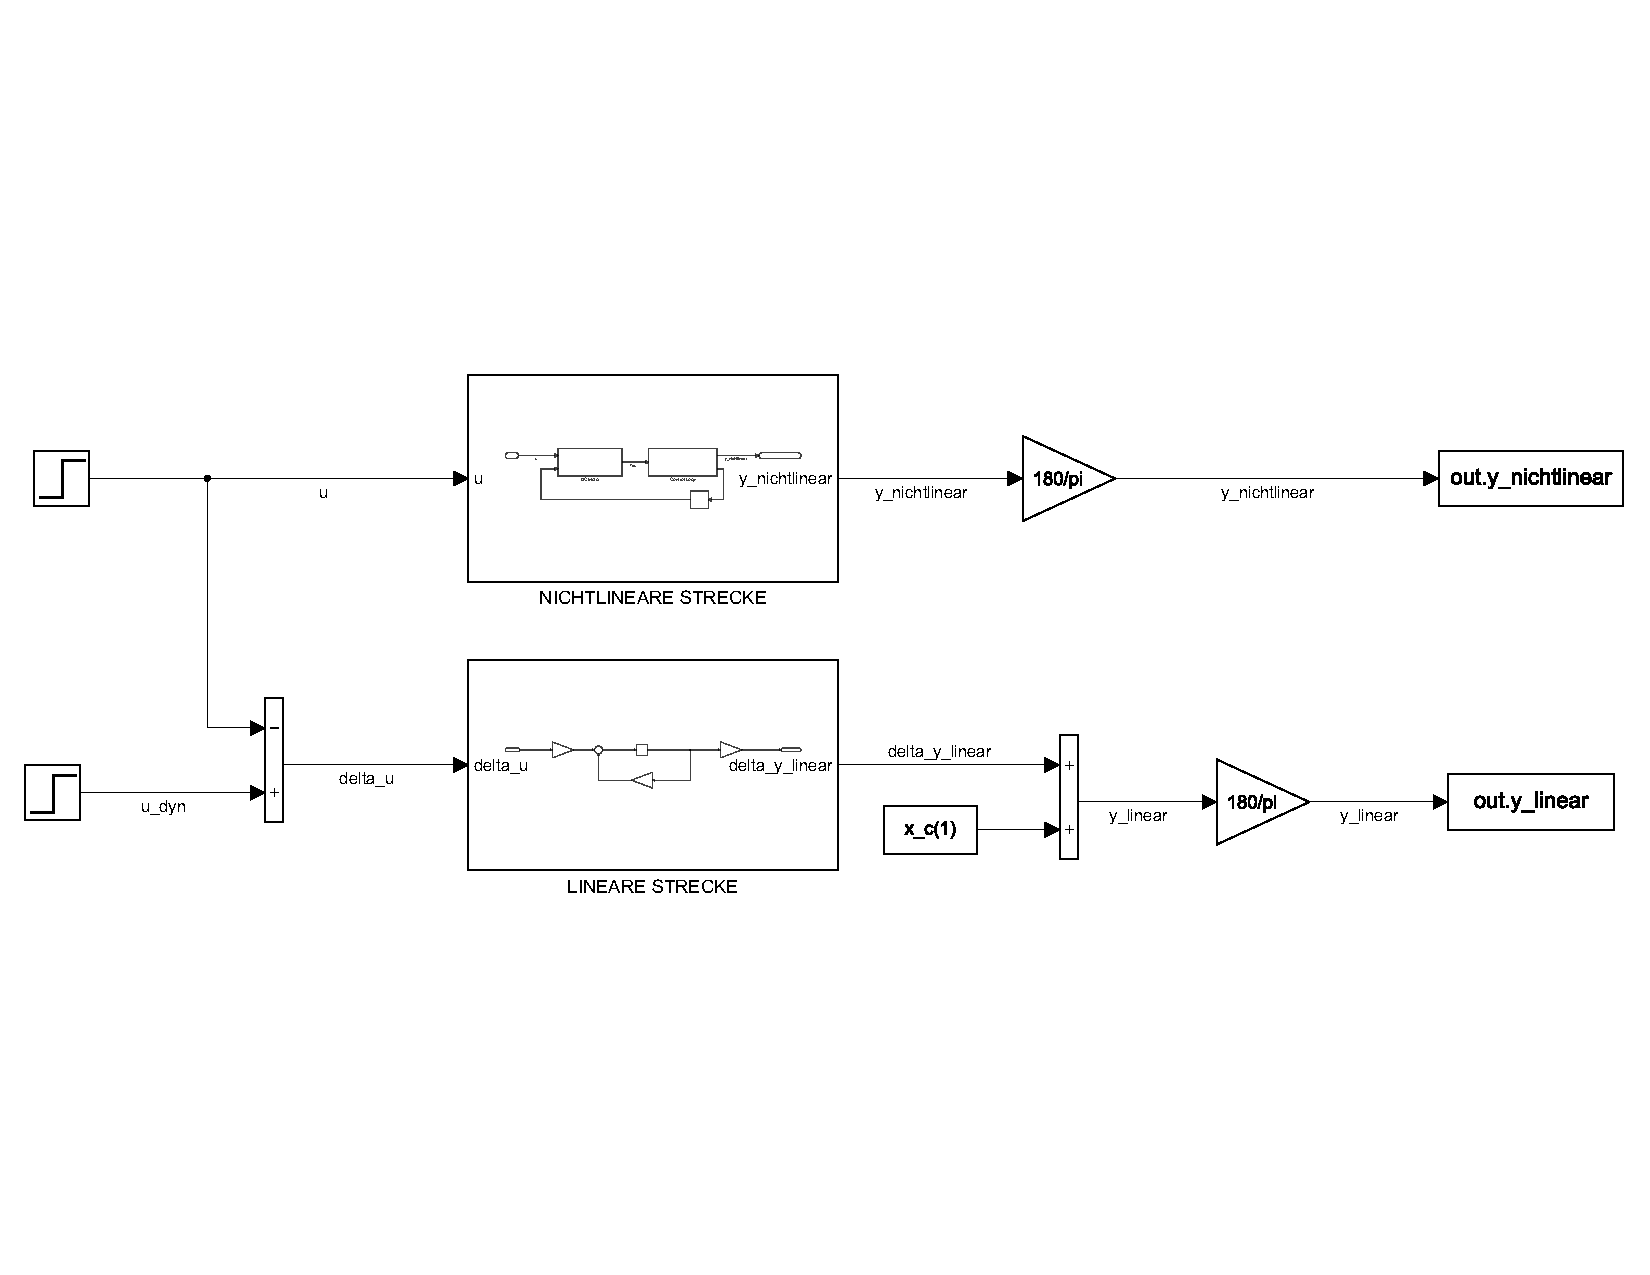
\includegraphics[width=0.65\textwidth]{Bilder/4. vergleich/system.pdf}}
   \caption[Übersicht der Simulationsstruktur]{Übersicht der Simulationsstruktur}
   \label{fig:Bild4.1}
\end{figure}

\begin{figure}[H]
   \centering
   \fbox{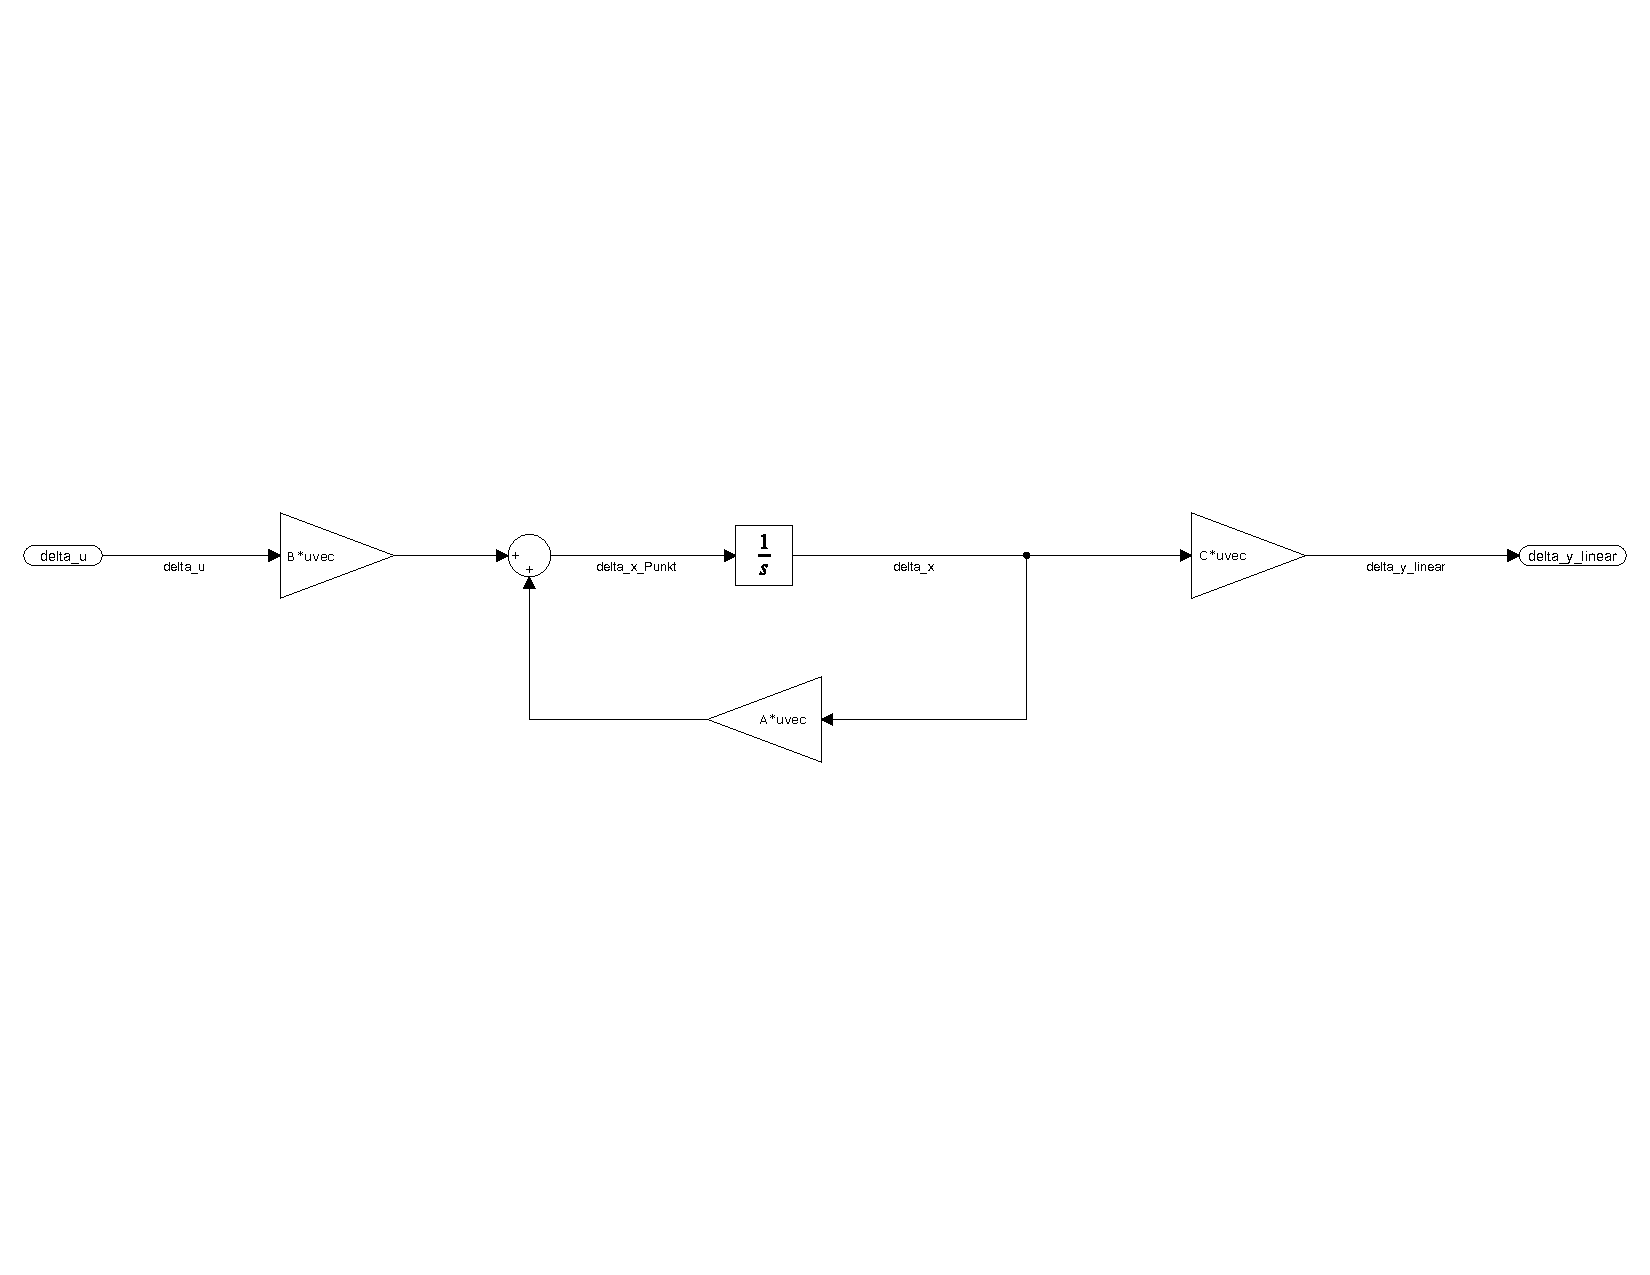
\includegraphics[width=0.65\textwidth]{Bilder/4. vergleich/linear.pdf}}
   \caption[Nichtlineare Strecke]{Nichtlineare Strecke}
   \label{fig:Bild4.2}
\end{figure}

\begin{figure}[H]
   \centering
   \fbox{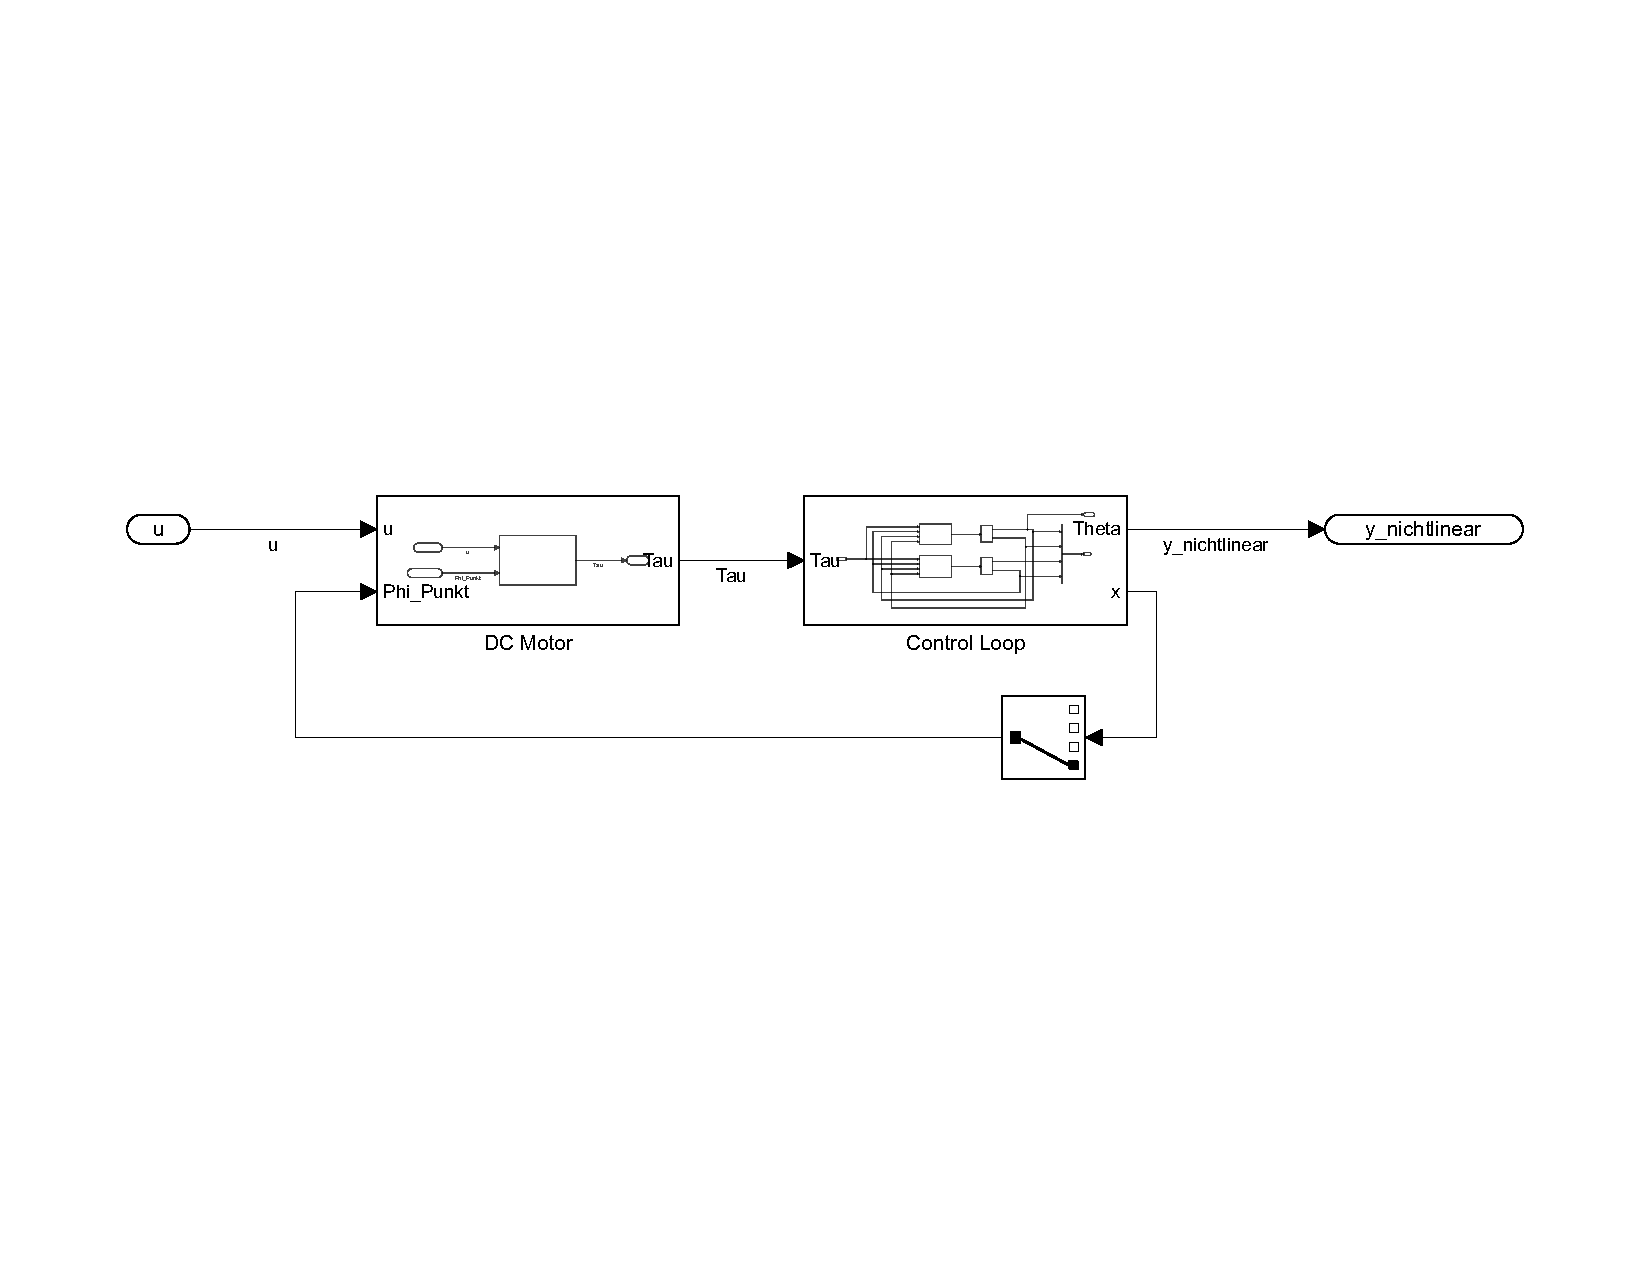
\includegraphics[width=0.65\textwidth]{Bilder/4. vergleich/nichtlinear.pdf}}
   \caption[Lineare Strecke]{Lineare Strecke}
   \label{fig:Bild4.3}
\end{figure}

Um das lineare mit dem nichtlinearen Modell zu vergleichen, werden gemäß \autoref{sec:Zustandsraumdarstellung} zu den Zuständen $\Delta \underline{x}$ die Ruhelagen $\underline{x}^*$ aus \autoref{eq:Gleichung3.10} addiert. Aus der \autoref{fig:Bild4.4} und \autoref{fig:Bild4.5} geht hervor, dass die implementierten Systeme für kleine Abweichungen von der Ruhelagen mit steigender Zeit $"t"$ selbiges Verhalten aufweisen.

\begin{figure}[H]
   \centering
   \fbox{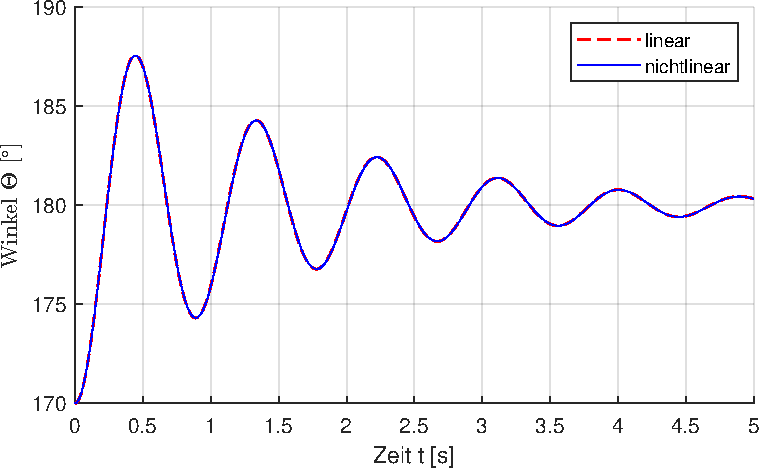
\includegraphics[width=0.7\textwidth]{Bilder/4. vergleich/vergleich_10_grad.pdf}}
   \caption[Vergleich der Pendelwinkel $\theta$ - kleine Auslenkung]{Vergleich der Pendelwinkel $\theta$ bei -10${^\circ}$ Anfangsauslenkung zur Ruhelage}
   \label{fig:Bild4.4}
\end{figure}

\begin{figure}[H]
   \centering
   \fbox{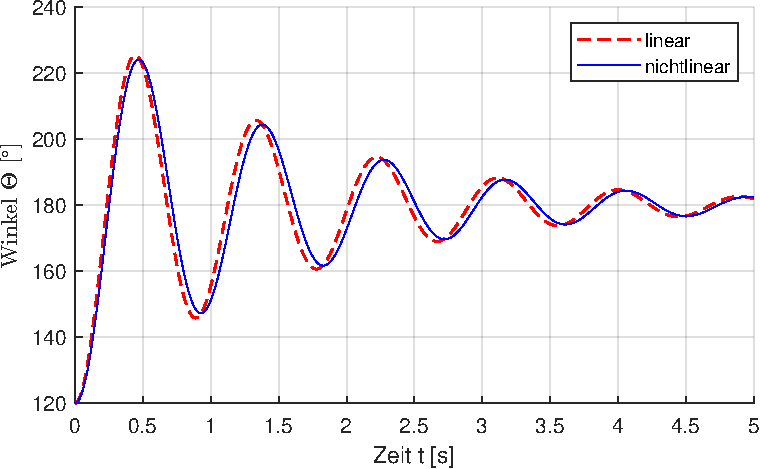
\includegraphics[width=0.7\textwidth]{Bilder/4. vergleich/vergleich_60_grad.pdf}}
   \caption[Vergleich der Pendelwinkel $\theta$ - große Auslenkung]{Vergleich der Pendelwinkel $\theta$ bei -60${^\circ}$ Anfangsauslenkung zur Ruhelage}
   \label{fig:Bild4.5}
\end{figure}

%\section{Zustandsreglerentwurf} \label{sec:Zustandsreglerentwurf}

\subsection{Einfache Zustandsrückführung} \label{sec:Einfach}

Auf Basis der Reglerstruktur aus \autoref{fig:Bild7} folgt das notwendige \textbf{Reglergesetz} zu

\begin{align}
    \underline{u}(t) &= -\underline{k}\cdot\underline{x}(t).
    \label{eq:Gleichung19}
\end{align}

\begin{figure}[H]
   \centering
   \fbox{\includegraphics[width=0.3\textwidth]{Bilder/5_zustandsreglerentwurf/Reglerstruktur_einfache_Zustandsrueckfuehrung.pdf}}
   \caption[Reglerstruktur der einfache Zustandsrückführung]{Reglerstruktur der einfachen Zustandsrückführung}
   \label{fig:Bild7}
\end{figure}

Die Berechnung der k-Faktoren wird mittels \textbf{linearen Matrixungleichungen} mithilfe von Matlab gelöst. Hierbei wird die exponentielle Stabilität mit der Decay-Rate $\alpha$ berücksichtigt. Das LMI wird formuliert über

\begin{align}
        \begin{split}
        \underline{X}\cdot \underline{A}^'+\underline{A}\cdot\underline{X} -\underline{M}^'\cdot\underline{B}^' - \underline{B}\cdot \underline{M} +2\cdot\alpha\cdot \underline{X} < 0 \\
    \underline{X} > 0
    \end{split}
    \label{eq:Gleichung20}
\end{align}
\newline
mit

\begin{align*}
    \underline{X} &= \underline{x} \quad X\in\mathbb{R}^{(2x1)}\\
    \underline{M} &= \underline{k}\cdot\underline{X} \quad M\in\mathbb{R}^{(1x2)}.
\end{align*}
\newline
Die \textbf{k-Faktoren} folgen aus: $k = M\cdot X^{-1}$. Die Decay-Rate wird mit 0.1 vorgesehen.

\begin{empheq}[box=\widefbox]{align}
    k &= 
    \begin{bmatrix}
        0.7112\cdot 10^{-3} & 0.0094\cdot 10^{-3}
    \end{bmatrix}
    \label{eq:Gleichung21}
\end{empheq}
Die Lage der Reglerpolstellen im Vergleich zu den Polstellen der Systemmatrix A sind in \autoref{fig:Bild8} visualisiert. Die Berechnung der \textbf{Reglerpolstellen} ist folgendermaßen definiert:

\begin{equation*}
    \boxed{sP = eig\left(\underline{A}-\underline{B}\cdot\underline{k}\right)}
\end{equation*}

\begin{figure}[H]
   \centering
   \fbox{\includegraphics[width=0.7\textwidth]{Bilder/5_zustandsreglerentwurf/Polstellen_einfache_Rueckfuehrung.pdf}}
   \caption[Polstellenlage der einfache Zustandsrückführung]{Polstellenlage der einfachen Zustandsrückführung im Vergleich zur Systemmatrix}
   \label{fig:Bild8}
\end{figure}

\subsection{Referenzwertvorsteuerung} \label{sec:Referenzwertvorsteuerung}

Die Reglerstruktur wird erweitert, sodass nun eine Referenzspannung vorgegeben werden kann. Diese wird mit einem Vorfilter F verrechnet (\autoref{fig:Bild9}).

\begin{figure}[H]
   \centering
   \fbox{\includegraphics[width=0.5\textwidth]{Bilder/5_zustandsreglerentwurf/Reglerstruktur_Vorsteuerung.pdf}}
   \caption[Reglerstruktur der Referenzwertvorsteuerung]{Reglerstruktur der Referenzwertvorsteuerung}
   \label{fig:Bild9}
\end{figure}

Das \textbf{Reglergesetz} resultiert zu

\begin{align}
    \underline{u}(t) &= -\underline{k}\cdot\underline{x}(t)+\underline{F}\cdot\underline{y}_{\mathrm{ref}(t)}.
    \label{eq:Gleichung22}
\end{align}
\newline
Die Berechnung der \textbf{k-Faktoren} erfolgt analog zum \autoref{sec:Einfach} mit einer Decay-Rate $\alpha = 0.1$.

\begin{empheq}[box=\widefbox]{align}
    k &= 
    \begin{bmatrix}
        -0.7112\cdot 10^{-3} & 0.0094\cdot 10^{-3}
    \end{bmatrix}
    \label{eq:Gleichung23}
\end{empheq}
\newline
Die \textbf{Reglerpolstellen} und die \textbf{Eigenwerte der Systemmatrix} werden in \autoref{fig:Bild10} dargelegt.

\begin{figure}[H]
   \centering
   \fbox{\includegraphics[width=0.7\textwidth]{Bilder/5_zustandsreglerentwurf/Polstellen_Referenzwertvorsteuerung.pdf}}
   \caption[Polstellenlage der Referenzwertvorsteuerung]{Polstellenlage der Referenzwertvorsteuerung im Vergleich zur Systemmatrix}
   \label{fig:Bild10}
\end{figure}

Die Berechnung des \textbf{Vorfilters} $F$ wird auf Grundlage der \autoref{eq:Gleichung24} durchgeführt und errechnet sich zu
\begin{align}
    \underline{F} &= \left(C_{\mathrm{Vor}}\cdot\left(-\underline{A}+\underline{B}\cdot\underline{k}\right)^{-1}\cdot\underline{B}\right)^{-1}
    \label{eq:Gleichung24}
\end{align}
\newline
mit

\begin{align*}
    C_{\mathrm{Vor}} &= 
    \begin{bmatrix}
        1 & 0
    \end{bmatrix}.
\end{align*}
\newline
Die Berechnung des Vorfilters ergibt

\begin{equation}
    \boxed{F = -1.0173\cdot 10^{-4}}.
\end{equation}

\subsection{I-Regelung} \label{sec:Iregler}

Das anzuwendende \textbf{Reglergesetz} folgt aus der Reglerstruktur in \autoref{fig:Bild11} und ergibt sich zu

\begin{align}
    \underline{u} &= \underline{k}_{\mathrm{I}}\cdot\int_{0}^t(\underline{y}_{\mathrm{ref}}-\underline{y})d\tau-\underline{k}_{\mathrm{x}}\cdot\underline{x}.
    \label{eq:Gleichung25}
\end{align}

\begin{figure}[H]
   \centering
   \fbox{\includegraphics[width=0.7\textwidth]{Bilder/5_zustandsreglerentwurf/Reglerstruktur_I_Regelung.pdf}}
   \caption[Reglerstruktur der I-Regelung]{Reglerstruktur der Regelung mit Integrationsglied}
   \label{fig:Bild11}
\end{figure}

Zur Vereinfachung wird nachfolgende Definition

\begin{align*}
    \underline{x}_{\mathrm{I}}& :=\int_{0}^t(\underline{y}_{\mathrm{ref}}-\underline{y})d\tau
\end{align*}
\newline
eingesetzt zu

\begin{align}
    \underline{u} &= \underline{k}_{\mathrm{I}}\cdot\underline{x}_{\mathrm{I}}-\underline{k}_{\mathrm{x}}\cdot\underline{x} \\ \nonumber \\
    \underline{u} &= -
    \begin{bmatrix}
        \underline{k}_{\mathrm{x}} & -\underline{k}_{\mathrm{I}}
    \end{bmatrix}
    \cdot
    \begin{bmatrix}
        \underline{x} \\
        \underline{x}_{\mathrm{I}}
    \end{bmatrix}
    \nonumber
\end{align}

mit
\begin{align}
    \underline{\tilde{k}} &= 
    \begin{bmatrix}
    \underline{k}_{\mathrm{x}} & -\underline{k}_{\mathrm{I}}
    \end{bmatrix}.
    \label{eq:Gleichung27}
\end{align}
Zur Berechnung der k-Faktoren wird ein \textbf{erweitertes Zustandsraummodell} eingeführt

\begin{align}
    \underline{\dot{\tilde{x}}} &= 
    \begin{bmatrix}
        \underline{A} & \underline{0} \\
        -\underline{C} & \underline{0}
    \end{bmatrix} \cdot \underline{\tilde{x}} +
    \begin{bmatrix}
        \underline{B} \\
        \underline{0}
    \end{bmatrix} \cdot\underline{u} +
    \begin{bmatrix}
        \underline{0} \\
        \underline{I}
    \end{bmatrix} \cdot\underline{y}_{ref}
    \label{eq:Gleichung28}
\end{align}
\newline
mit

\begin{align*}
    \underline{\tilde{A}} &= 
    \begin{bmatrix}
        \underline{A} & \underline{0} \\
        -\underline{C} & \underline{0}
    \end{bmatrix} \quad ; \underline{\tilde{A}}\in\mathbb{R}^{(n+p)x(n+p)}\\
    \underline{\tilde{B}} &= 
    \begin{bmatrix}
        \underline{B} \\
        \underline{0}
    \end{bmatrix}\qquad ; \underline{\tilde{B}}\in\mathbb{R}^{(n+p)x(m)}\\
    \underline{\tilde{B}}_{\mathrm{y}} &= 
    \begin{bmatrix}
        \underline{0} \\
        \underline{I}
    \end{bmatrix}\qquad  ;\underline{\tilde{B}}_{\mathrm{y}}\in\mathbb{R}^{(n+p)x(p)}.
\end{align*}
\newline
Die Matrix C wird wie in \autoref{sec:Referenzwertvorsteuerung} definiert. Somit folgen die Matrizen $\tilde{A}$ und $\tilde{B}$ nach der Definition zu:

\begin{empheq}[box=\widefbox]{align}
    \tilde{A} &=
    \begin{bmatrix}
        -150.4187 & -54.5419 & 0 \\
        486.5101 & 0 & 0 \\
        -1 & 0 & 0
    \end{bmatrix} \\
    \tilde{B} &=
    \begin{bmatrix}
        -2.1763\cdot 10^5 \\
        5.9499\cdot 10^5 \\
        0
    \end{bmatrix}
\end{empheq}
\newline
Die anschließende Berechnung der notwendigen \textbf{k-Faktoren} erfolgt analog zu \autoref{sec:Referenzwertvorsteuerung} mit den Tilde-Matrizen und $X\in\mathbb{R}^{(3x1)}$ und $M\in\mathbb{R}^{(1x3)}$. Die Decay-Rate wird auf 0.1 festgelegt.

\begin{empheq}[box=\widefbox]{align}
    k &=
    \begin{bmatrix}
        0.6921\cdot 10^{-3} & -0.0034\cdot 10^{-3} & 0.0497\cdot 10^{-3}
    \end{bmatrix}
    \label{eq:Gleichung29}
\end{empheq}
\newline
Zur Veranschaulichung der \textbf{Polstellenlagen} dient \autoref{fig:Bild12}.

\begin{figure}[H]
   \centering
   \fbox{\includegraphics[width=0.7\textwidth]{Bilder/5_zustandsreglerentwurf/Polstellen_I_Regelung.pdf}}
   \caption[Polstellenlage der Referenzwertvorsteuerung mit I-Anteil]{Polstellenlage der Referenzwertvorsteuerung mit I-Anteil im Vergleich zur Systemmatrix}
   \label{fig:Bild12}
\end{figure}

%\section{Reglervalidierung} \label{sec:Reglervalidierung}

Nachdem im vorangegangenen Abschnitt die Regler mit einfacher Zustandsrückführung, mit Referenzwertvorsteuerung und mit I-Regelung entworfen wurden, soll deren Funktionalität nun validiert werden. Dazu werden diese in Simulink implementiert und mit der Regelstrecke gekoppelt. Validiert wird gegen das lineare und das nicht-lineare Zustandsraummodell aus \autoref{sec:Zustandsraumdarstellung}. Die in \autoref{sec:Zustandsreglerentwurf} berechneten Reglerparameter (\zB k-Faktoren) werden in Simulink eingesetzt. Anschließend sollen die Simulationsergebnisse auf ihre Plausibilität geprüft und das Regelverhalten bewertet werden. 

\subsection{Validierung des linearen Modells} \label{sec:Vergleich_linear}

Begonnen wird mit der Reglervalidierung am linearen Zustandsraummodell. Die lineare Strecke wurde bereits in Simulink umgesetzt und ist in \autoref{fig:Bild4} dargestellt. Bei der Umsetzung der Regler am linearen Modell ist wichtig zu beachten, dass nicht nur der Regler mit Delta-Größen arbeitet, sondern auch die Regelstrecke Delta-Zustandsgrößen erwartet und ausgibt. Folglich müssen für die Ausgabe der Zustandsvektoren $v_{\mathrm{PV}}$ und $i_{\mathrm{L}}$ und der Eingangsgröße $u$ in Diagrammform die Ruhelagen \bzw der Duty Cycle $d$ addiert werden.

\subsubsection{Zustandsregler mit einfacher Zustandsrückführung}

Als erster Regler wurde der Zustandsregler mit einfacher Rückführung umgesetzt. Das Simulink-Blockschaltbild ist in \autoref{fig:Bild13} gezeigt. Simuliert werden die Zustandsgrößen $v_{\mathrm{PV}}$ und $i_{\mathrm{L}}$ sowie die Eingangsgröße $u$ bei $\alpha = 0.1$ für die Berechnung der k-Faktoren mit LMI's (siehe \autoref{eq:Gleichung21}).

\begin{figure}[H]
    \centering
    \fbox{\includegraphics[width=0.65\textwidth]{Bilder/6_reglervalidierung/linear_einfacher_regler_simu.pdf}}
    \caption[Einfacher Zustandsregler Simulink (linear)]{Simulink Regler-Blockschaltbild für den einfachen Zustandsregler (lineares Zustandsraummodell)}
    \label{fig:Bild13}
\end{figure}

Zur Validierung der Funktionsfähigkeit des Reglers wird der Anfangswert der Spannung $v_{\mathrm{PV}}$ um $\SI{10}{V}$ bezogen auf die Ruhelage der PV-Spannung $v_{\mathrm{PV,MPP}}$ abgesenkt. \autoref{fig:Bild14} zeigt, dass der Regler fähig ist, das System wieder in die Ruhelage zu regeln. Dabei wird die Begrenzung der Eingangsgröße $u$, welche zwischen maximal 0 und 1 liegen darf aufgrund der Definition des Duty Cycles, nicht über- oder unterschritten.

\begin{figure}[H]
    \centering
    \fbox{\includegraphics[width=0.85\textwidth]{Bilder/6_reglervalidierung/linear_einfache_rueckfuehrung.pdf}}
    \caption[Validierung Regler mit einfacher Rückführung (linear)]{$v_{\mathrm{PV}}$, $i_{\mathrm{L}}$ und $u$ bei $\alpha = 0.1$ und einem Einganssprung von $v_{\mathrm{PV,MPP}} - \SI{10}{V}$ am einfachen Zustandsregler für das lineare Zustandsraummodell}
    \label{fig:Bild14}
\end{figure}

Es fällt jedoch auf, dass das System stark schwingt und unter anderem dadurch \ca $\SI{8}{s}$ benötigt, um bei einer kleinen initialen Spannungsabweichung wieder zurück in die Ruhelage geregelt zu werden. Das beschriebene Verhalten kann als plausibel erachtet werden, da der Betrag des Imaginärteils der Polstellen um einen Faktor 50 größer ist als der Betrag des Realteils der Polstellen, was aus \autoref{fig:Bild8} hervorgeht. Auf eine Verbesserung dieses Verhaltens über die Anpassung der LMI's wird an dieser Stelle verzichtet. Es konnte nachgewiesen werden, dass der Regler grundsätzlich seine Funktion erfüllt.

\subsubsection{Zustandsregler mit Vorsteuerung} \label{sec:val_lin_vor}

Als nächster Regler wird der Zustandsregler mit Referenzwertvorsteuerung behandelt. Dessen Umsetzung in Simulink kann in \autoref{fig:Bild15} nachvollzogen werden. Ebenfalls wieder simuliert, werden die Zustandsgrößen $v_{\mathrm{PV}}$ und $i_{\mathrm{L}}$ sowie die Eingangsgröße $u$ bei $\alpha = 0.1$ für die Berechnung der k-Faktoren mit LMI's (siehe \autoref{eq:Gleichung23}). Im Unterschied zum vorangegangenen Regler soll es nun auch möglich sein, einen Referenzwert für die PV-Spannung vorzugeben. Dazu wurde in \autoref{eq:Gleichung24} ein Vorfilter $F$ berechnet, über welchen ein Referenzwert $y_{\mathrm{ref}}$ vorgegeben werden kann.

\begin{figure}[H]
    \centering
    \fbox{\includegraphics[width=1.0\textwidth]{Bilder/6_reglervalidierung/linear_vorsteuerung_simu.pdf}}
    \caption[Zustandsregler mit Vorsteuerung Simulink (linear)]{Simulink Regler-Blockschaltbild für den Zustandsregler mit Vorsteuerung (lineares Zustandsraummodell)}
    \label{fig:Bild15}
\end{figure}

Zur Validierung der Funktionsfähigkeit des Reglers wird ein Referenzwert von $\SI{+10}{V}$ bezogen für die PV-Spannung $v_{\mathrm{PV,MPP}}$ vorgegeben. \autoref{fig:Bild16} zeigt, dass der Regler fähig ist das System zum angegeben Referenzwert auszuregeln. Dabei wird die Begrenzung der Eingangsgröße von $u \in \mathbb{R} \: | \: 0 \leq u \leq 1$ nicht über- oder unterschritten. \\
Auch hier fällt auf, dass das System stark schwingt und erneut rund $\SI{8}{s}$ benötigt, um den gewünschten Referenzwert zu erreichen. Die Begründung findet sich ebenfalls in der Lage der Polstellen, bei welchen der Betrag des Imaginärteils 50-fach größer ist als der Betrag des Realteils (siehe \autoref{fig:Bild10}).

\begin{figure}[H]
    \centering
    \fbox{\includegraphics[width=0.85\textwidth]{Bilder/6_reglervalidierung/linear_referenzwertvorsteuerung.pdf}}
    \caption[Validierung Regler mit Vorsteuerung (linear)]{$v_{\mathrm{PV}}$, $i_{\mathrm{L}}$ und $u$ bei $\alpha = 0.1$ und einem Referenzwert von $y_{ref} = v_{\mathrm{PV,MPP}} + \SI{10}{V}$ am Zustandsregler mit Referenzwertvorsteuerung für das lineare Zustandsraummodell}
    \label{fig:Bild16}
\end{figure}

\subsubsection{Zustandsregler mit I-Regelung}

Der dritte umgesetzte Zustandsregler ist der I-Regler. Die Implementation für Simulink ist in \autoref{fig:Bild17} dargestellt. Auch hier werden die Zustandsgrößen $v_{\mathrm{PV}}$ und $i_{\mathrm{L}}$ sowie die Eingangsgröße $u$ bei $\alpha = 0.1$ für die Berechnung der k-Faktoren mit LMI's (siehe \autoref{eq:Gleichung29}) simuliert. Abweichend zu den vorherigen Reglern wird zunächst das erweiterte Zustandsraummodell aufgestellt (\autoref{eq:Gleichung28}), über welches die Tilde-Matrizen für die A- und B-Matrix erhalten werden können. Mit Hilfe dieser werden nun drei statt zwei k-Faktoren über LMI's berechnet. Wie auch schon bei der Referenzwertvorsteuerung ist es möglich einen Referenzwert $y_{\mathrm{ref}}$ vorzugeben. Der wesentliche Unterschied zur Vorsteuerung liegt im Aufintegrieren des Regelfehlers, wodurch eine generelle Optimierung des Regelverhaltens zu erwarten ist.

\begin{figure}[H]
    \centering
    \fbox{\includegraphics[width=1.0\textwidth]{Bilder/6_reglervalidierung/linear_i_regler_simu.pdf}}
    \caption[Zustandsregler mit I-Regelung Simulink (linear)]{Simulink Regler-Blockschaltbild für den Zustandsregler mit I-Regelung (lineares Zustandsraummodell)}
    \label{fig:Bild17}
\end{figure}

Zur Validierung der Funktionsfähigkeit des Reglers wird erneut ein Referenzwert von $\SI{+10}{V}$ bezogen für die PV-Spannung $v_{\mathrm{PV,MPP}}$ vorgegeben. \autoref{fig:Bild18} zeigt, dass der Regler fähig ist das System zum angegeben Referenzwert auszuregeln. Dabei wird die Begrenzung der Eingangsgröße von $u \in \mathbb{R} \: | \: 0 \leq u \leq 1$ nicht über- oder unterschritten. \\
Es kann positiv vermerkt werden, dass das System im Vergleich zu den vorangegangenen Reglern nur noch minimal schwingt. Grund dafür ist vermutlich die dritte Polstelle (siehe \autoref{fig:Bild12}), die im Vergleich zu den ersten beiden keinen Imaginärteil aufweist und damit das System weniger schwingungsfähig macht. Begründet durch die höhere Komplexität des Reglers dauert der Vorgang des Ausregelns zu dem gewünschten Referenzwert jedoch \ca $\SI{2}{s}$ länger als beim Zustandsregler mit Referenzwertvorsteuerung.

\begin{figure}[H]
    \centering
    \fbox{\includegraphics[width=0.85\textwidth]{Bilder/6_reglervalidierung/linear_i_regelung.pdf}}
    \caption[Validierung Regler mit I-Regelung (linear)]{$v_{\mathrm{PV}}$, $i_{\mathrm{L}}$ und $u$ bei $\alpha = 0.1$ und einem Referenzwert von $y_{ref} = v_{\mathrm{PV,MPP}} + \SI{10}{V}$ am Zustandsregler mit I-Regelung für das lineare Zustandsraummodell}
    \label{fig:Bild18}
\end{figure}

\subsubsection{Vergleich des Regelverhaltens}

Abschließend wird ein Vergleich der drei Regelkonzepte für das lineare Zustandsraummodell vorgenommen. Dabei werden die Regler bezüglich der Performance gegenübergestellt. Um einen konkreten Vergleich vornehmen zu können, wurden die Kurvenverläufe, die bereits auf den vorhergehenden Seiten gezeigt worden sind, für die Größen $v_{\mathrm{PV}}$, $i_{\mathrm{L}}$ und $u$ übereinander gelegt. \autoref{fig:Bild19} zeigt den Vergleich der drei Zustandsregler. \\
\newline
Es ist zunächst offensichtlich, dass ein wesentlicher Unterschied zwischen dem Regler mit einfacher Zustandsrückführung und den beiden Reglern mit der Fähigkeit einen Referenzwert entgegenzunehmen besteht. Durch die Referenzwertvorgabe für die Spannung $v_{\mathrm{PV}}$ bei einem Referenzwert von $\SI{+10}{V}$ bezogen für die PV-Spannung $v_{\mathrm{PV,MPP}}$ ist der Endwert für den Zustandsregler mit Vorsteuerung und für den Zustandsregler mit I-Regelung um $\SI{10}{V}$ größer. Dies ist im Spannungsdiagramm in \autoref{fig:Bild19} ersichtlich.\\
Durch die angepasste Spannung ändert sich auch der Strom $i_{\mathrm{L}}$ und der Eingang $u$ anti-proportional zu der Differenz des Referenzwertes bezogen auf die Ruhelage.\\
\newline
Weiterhin ist zu erkennen, dass die Geschwindigkeit der drei Regler voneinander abweicht, obwohl für die Berechnung der k-Faktoren der Zustandsregler das selbe $\alpha$ ($\alpha = 0.1$) verwendet wurde. In der \autoref{fig:Bild19} ist zu erkennen, dass die Hüllkurve des einfachen Zustandsreglers und die des Reglers mit Vorsteuerung annähernd identisch sind. Vergleicht man diese jedoch mit dem Kurvenverlauf des I-Reglers kann ermittelt werden, dass dieser, was das Ausregeln der Zustandsgröße $v_{\mathrm{PV}}$ angeht, etwas langsamer scheint. Dieses Phänomen ergibt sich vermutlich aus dem weiteren k-Faktor bei der I-Regelung und der damit einhergehenden erhöhten Komplexität, nicht zuletzt auch durch die ebenfalls dazugekommene Integration.\\
\newline
Bei der Betrachtung des Zustandsreglers mit I-Regelung im Vergleich zu den anderen beiden Regelkonzepten fällt auf, dass die Schwingungen stark reduziert sind. Dabei handelt es sich um einen wünschenswerten Effekt, der maßgeblich durch die Polstellenlage beeinflusst wird. Der I-Regler besitzt eine weitere Polstelle, welche rein reell ist und damit dämpfend gegenüber den Polstellen mit großem Imaginärteil wirkt.

\begin{figure}[H]
    \centering
    \fbox{\includegraphics[width=0.8\textwidth]{Bilder/6_reglervalidierung/linear_reglervergleich.pdf}}
    \caption[Reglervergleich für das lineare Zustandsraummodell]{$v_{\mathrm{PV}}$, $i_{\mathrm{L}}$ und $u$ für Regler mit einfacher Zustandsrückführung, Regler mit Referenzwertvorsteuerung und Regler mit I-Regelung bei einem Einganssprung von $v_{\mathrm{PV,MPP}} - \SI{10}{V}$ \bzw einem Referenzwert von $y_{ref} = v_{\mathrm{PV,MPP}} + \SI{10}{V}$ am linearen Zustandsraummodell}
    \label{fig:Bild19}
\end{figure}

\subsection{Validierung des nichtlinearen Modells} \label{sec:Vergleich_nichtlinear}

Der zweite Unterabschnitt behandelt die Validierung der Regler am nichtlinearen Zustandsraummodell. Die nichtlineare Strecke wurde bereits in Simulink umgesetzt und ist in \autoref{fig:Bild3} dargestellt. Bei der Umsetzung der Regler für das nichtlinearen Modell ist wichtig zu beachten, dass ausschließlich der Regler mit Delta-Größen arbeitet, die Regelstrecke im Vergleich zum linearen Modell jedoch nicht. Für die Ausgabe der Zustandsvektoren $v_{\mathrm{PV}}$ und $i_{\mathrm{L}}$ in Diagrammform können direkt die Ausgänge der Regelstrecke visualisiert werden. Die Eingangsgröße $u$ muss weiterhin mit dem Duty Cycle $d$ verrechnet werden. Da die Zustandsvektoren auf den Regler zurückgeführt sind, muss am Eingang des Reglers die jeweilige Ruhelage subtrahiert werden. Dieser Zusammenhang ist beispielsweise in \autoref{fig:Bild20} auf der linken Seite zu erkennen. 

\subsubsection{Zustandsregler mit einfacher Zustandsrückführung}

Erneut wird mit dem Zustandsregler mit einfacher Rückführung begonnen. Das Simulink-Blockschaltbild ist in \autoref{fig:Bild20} gezeigt. Simuliert werden die Zustandsgrößen $v_{\mathrm{PV}}$ und $i_{\mathrm{L}}$ sowie die Eingangsgröße $u$ bei $\alpha = 0.1$ für die Berechnung der k-Faktoren mit LMI's (siehe \autoref{eq:Gleichung21}).

\begin{figure}[H]
    \centering
    \fbox{\includegraphics[width=1.0\textwidth]{Bilder/6_reglervalidierung/nichtlinear_einfacher_regler_simu.pdf}}
    \caption[Einfacher Zustandsregler Simulink (nicht-linear)]{Simulink Regler-Blockschaltbild für den einfachen Zustandsregler (nichtlineares Zustandsraummodell)}
    \label{fig:Bild20}
\end{figure}

Zur Validierung der Funktionsfähigkeit des Reglers wird der Anfangswert der Spannung $v_{\mathrm{PV}}$ um $\SI{10}{V}$ bezogen auf die Ruhelage der PV-Spannung $v_{\mathrm{PV,MPP}}$ abgesenkt. \autoref{fig:Bild21} zeigt nahezu identische Ergebnisse im Vergleich zum linearen Zustandsraummodell. Aufgrund dieser Erkenntnis wird auf weitere Analysen verzichtet.

\begin{figure}[H]
    \centering
    \fbox{\includegraphics[width=0.85\textwidth]{Bilder/6_reglervalidierung/nichtlinear_einfache_rueckfuehrung.pdf}}
    \caption[Validierung Regler mit einfacher Rückführung (nichtlinear)]{$v_{\mathrm{PV}}$, $i_{\mathrm{L}}$ und $u$ bei $\alpha = 0.1$ und einem Einganssprung von $v_{\mathrm{PV,MPP}} - \SI{10}{V}$ am einfachen Zustandsregler für das nichtlineare Zustandsraummodell}
    \label{fig:Bild21}
\end{figure}

\subsubsection{Zustandsregler mit Vorsteuerung} \label{sec:val_nlin_vor}

Nachfolgend wird der Zustandsregler mit Referenzwertvorsteuerung auf das nichtlineare Zustandsraummodell angewendet. Die Umsetzung des Reglers in Simulink kann in \autoref{fig:Bild22} nachvollzogen werden. Ebenfalls wieder simuliert, werden die Zustandsgrößen $v_{\mathrm{PV}}$ und $i_{\mathrm{L}}$ sowie die Eingangsgröße $u$ bei $\alpha = 0.1$ für die Berechnung der k-Faktoren mit LMI's (siehe \autoref{eq:Gleichung23}). Im Unterschied zum vorangegangenen Regler Soll es nun auch möglich sein, einen Referenzwert für die PV-Spannung vorzugeben. Dazu wurde in \autoref{eq:Gleichung24} ein Vorfilter $F$ berechnet, über welchen ein Referenzwert $y_{\mathrm{ref}}$ vorgegeben werden kann.

\begin{figure}[H]
    \centering
    \fbox{\includegraphics[width=1.0\textwidth]{Bilder/6_reglervalidierung/nichtlinear_vorsteuerung_simu.pdf}}
    \caption[Zustandsregler mit Vorsteuerung Simulink (nichtlinear)]{Simulink Regler-Blockschaltbild für den Zustandsregler mit Vorsteuerung (nichtlineares Zustandsraummodell)}
    \label{fig:Bild22}
\end{figure}

Bei der Betrachtung der Ergebnisse aus \autoref{fig:Bild23} fällt auf, dass sowohl die Spannung $v_{\mathrm{PV}}$, der Strom $i_{\mathrm{L}}$ und der Eingang $u$ von den Simulationsergebnissen aus \autoref{sec:val_lin_vor} signifikant abweichen. Das System schwingt nur kurz und ist in unter $\SI{500}{ms}$ zum Referenzwert ausgeregelt. Es scheint, als wäre die Performance des Reglers stark gesteigert. Es handelt sich jedoch vermutlich um die Auswirkungen des Regelfehlers bei der Referenzwertvorsteuerung, welche sich offensichtlich positiv auf das Regelverhalten auswirken.

\begin{figure}[H]
    \centering
    \fbox{\includegraphics[width=0.85\textwidth]{Bilder/6_reglervalidierung/nichtlinear_referenzwertvorsteuerung.pdf}}
    \caption[Validierung Regler mit Vorsteuerung (nichtlinear)]{$v_{\mathrm{PV}}$, $i_{\mathrm{L}}$ und $u$ bei $\alpha = 0.1$ und einem Referenzwert von $y_{ref} = v_{\mathrm{PV,MPP}} + \SI{10}{V}$ am Zustandsregler mit Referenzwertvorsteuerung für das nichtlineare Zustandsraummodell}
    \label{fig:Bild23}
\end{figure}

\subsubsection{Zustandsregler mit I-Regelung}

Der zuletzt umgesetzte Zustandsregler ist der I-Regler für das nichtlineare Zustandsraummodell. Die Implementation für Simulink ist in \autoref{fig:Bild24} dargestellt. Auch hier werden die Zustandsgrößen $v_{\mathrm{PV}}$ und $i_{\mathrm{L}}$ sowie die Eingangsgröße $u$ bei $\alpha = 0.1$ für die Berechnung der k-Faktoren mit LMI's (siehe \autoref{eq:Gleichung29}) simuliert. Abweichend zu den vorherigen Reglern wird zunächst das erweiterte Zustandsraummodell aufgestellt (\autoref{eq:Gleichung28}), über welches die Tilde-Matrizen für die A- und B-Matrix erhalten werden können. Mit Hilfe dieser werden nun drei statt zwei k-Faktoren über LMI's berechnet. Wie auch schon bei der Referenzwertvorsteuerung ist es möglich einen Referenzwert $y_{\mathrm{ref}}$ vorzugeben. Der wesentliche Unterschied zur Vorsteuerung liegt im Aufintegrieren des Regelfehlers, wodurch eine generelle Optimierung des Regelverhaltens zu erwarten ist.

\begin{figure}[H]
    \centering
    \fbox{\includegraphics[width=1.0\textwidth]{Bilder/6_reglervalidierung/nichtlinear_i_regler_simu.pdf}}
    \caption[Zustandsregler mit I-Regelung Simulink (nichtlinear)]{Simulink Regler-Blockschaltbild für den Zustandsregler mit I-Regelung (nichtlineares Zustandsraummodell)}
    \label{fig:Bild24}
\end{figure}

Zur Validierung der Funktionsfähigkeit des Reglers wird erneut ein Referenzwert von $\SI{+10}{V}$ bezogen für die PV-Spannung $v_{\mathrm{PV,MPP}}$ vorgegeben. \autoref{fig:Bild25} zeigt nahezu identische Ergebnisse im Vergleich zum linearen Zustandsraummodell. Aufgrund dieser Erkenntnis wird auf weitere Analysen verzichtet.

\begin{figure}[H]
    \centering
    \fbox{\includegraphics[width=0.85\textwidth]{Bilder/6_reglervalidierung/nichtlinear_i_regelung.pdf}}
    \caption[Validierung Regler mit I-Regelung (nichtlinear)]{$v_{\mathrm{PV}}$, $i_{\mathrm{L}}$ und $u$ bei $\alpha = 0.1$ und einem Referenzwert von $y_{ref} = v_{\mathrm{PV,MPP}} + \SI{10}{V}$ am Zustandsregler mit I-Regelung für das nichtlineare Zustandsraummodell}
    \label{fig:Bild25}
\end{figure}

\subsubsection{Vergleich des Regelverhaltens}

Abschließend kann festgehalten werden, dass die drei entwickelten Regler auch auf das nichtlineare Zustandsraummodell angewendet werden können und grundsätzlich plausible Ergebnisse produzieren. Bei der Referenzwertvorgabe für den Regler mit Vorsteuerung \bzw Regler mit I-Regelung konnte quantitativ ermittelt werden, dass die Performance der Zustandsregler nur für Referenzwerte von $y_{\mathrm{ref}} \in \mathbb{R} \: | \: \SI{-9}{V} \leq y_{\mathrm{ref}} \leq \SI{+12}{V}$ ausreicht. \\
Bis auf die Regelung mit Referenzwertvorsteuerung konnten annähern identische Kurvenverläufe im Vergleich zu den Simulationen am linearen Modell festgestellt werden. Besagte Unterschiede wurden bereits in \autoref{sec:val_nlin_vor} analysiert und festgehalten. Somit wird auf weitere Vergleiche an dieser Stelle verzichtet.

\begin{figure}[H]
    \centering
    \fbox{\includegraphics[width=0.8\textwidth]{Bilder/6_reglervalidierung/nichtlinear_reglervergleich.pdf}}
    \caption[Reglervergleich für das nichtlineare Zustandsraummodell]{$v_{\mathrm{PV}}$, $i_{\mathrm{L}}$ und $u$ für Regler mit einfacher Zustandsrückführung, Regler mit Referenzwertvorsteuerung und Regler mit I-Regelung bei einem Einganssprung von $v_{\mathrm{PV,MPP}} - \SI{10}{V}$ \bzw einem Referenzwert von $y_{ref} = v_{\mathrm{PV,MPP}} + \SI{10}{V}$ am nichtlinearen Zustandsraummodell}
    \label{fig:Bild26}
\end{figure}

%\section{Ausblick} \label{sec:ausblick}

Wie bereits in \autoref{sec:Reglervalidierung} aufgefallen ist, schwingt das System sehr stark bei Reglern mit einfacher Zustandsrückführung und Zustandsreglern mit Referenzwertvorsteuerung. Grund dafür ist der Betrag des Imaginärteils der Polstellen, welcher um ein Vielfaches größer ist als der Betrag des Realteils. Um den Imaginärteil zu verkleiner besteht die Möglichkeit die Polregion über LMI's weiter einzuschränken. Der aktuelle Ansatz nutzt lediglich eine Einschränkung über die Vorgabe eines $\alpha$-Wertes, um die Polstellen links einer vorgegebenen Position auf der Real-Achse zu platzieren. Dies zwingt das System in einen stabilen Zustand.\\
Das bisherige LMI könnte über zusätzliche Vorgaben erweitert werden, um die Polregion zu verkleinern \bzw zu optimieren. Dazu wird ein Parameter $r$ für die Auslegung eines Kreisradius um den Koordinatenursprung eingeführt sowie ein $\theta$, um einen Sektor links der Imaginärachse über die Wahl eines Winkels festzulegen. Die sich ergebende Polregion ist in \autoref{fig:Bild27} dargestellt.\\

\begin{figure}[H]
    \centering
    \begin{tikzpicture}[framed][domain=0:0]
        \draw[very thin,color=black] (-0.1,-1.1);                               % Umgebung
        \draw[dashed] (0,-3) arc(270:90:3) -- cycle;                            % Halbkreis
        \draw[-stealth] (0,0) -- (-1.24,2.74);                                  % r-Pfeil
        \node[text width=1cm] at (0, 1.6) {$r$};                                % r
        \draw[dashed] (-0.8,-4) -- (-0.8,4);                                    % alpha-Grenze
        \draw[dashed] (0,0) -- (-3,3);                                          % +theta-Grenze
        \draw[dashed] (0,0) -- (-3,-3);                                         % -theta-Grenze
        \draw[-stealth] (0,-2.5) -- (-0.8,-2.5) node[midway, above] {$\alpha$}; % alpha-Pfeil
        \node[text width=1cm] at (0.6, -0.3) {0};                               % Koordinatenursprung
        \draw[-stealth] (-0.7,0) to [bend left] (-0.5,0.5);                     % theta-Pfeil
        \node[text width=1cm] at (-0.1, 0.2) {$\theta$};                        % theta
        \begin{scope}
            \clip (-5,-4) rectangle (-0.8,4);                                   % Clipping Maske zur Begrenzung des Bereichs
            \draw[pattern={crosshatch}, pattern color=grey] (0,0) -- (-2.12,2.12) arc[start angle=135, delta angle=90,radius=3] -- (0,0); % gefüllter Bereich
        \end{scope}
        \draw[] (-0.8,-0.8) -- (-0.8,0.8);                                      % Begrenzung rechte Seite des Bereichs
        \node[text width=3cm] at (-1.2,0.5) {$S(\alpha,r,\theta)$};             % Beschriftung Bereich
        \draw[->] (-4.2,0) -- (2,0) node[right] {$Re$};                         % X-Achse
        \draw[->] (0,-4) -- (0,4) node[above] {$Im$};                           % Y-Achse
    \end{tikzpicture}
    \caption[Polregion bei erweitertem LMI]{Polregion bei Erweiterung des LMI zu $S(\alpha,r,\theta)$}
    \label{fig:Bild27}
\end{figure}

\clearpage

Die Formulierung der erweiterten LMI's ist nachfolgend dargestellt:\\
\begin{align*}
    \begin{split}
        0 &> AX + XA^T - BM -M^TB^T + 2\alpha X\\\\
        0 &>
        \begin{pmatrix}
            (AX + XA^T - BM - M^TB^T)\sin\theta & (AX - XA^T - BM + M^TB^T)\cos\theta \\\\
            (XA^T - AX - BM - M^TB^T)\cos\theta & (AX + XA^T - BM - M^TB^T)\sin\theta
        \end{pmatrix}\\\\
        0 &> 
        \begin{pmatrix}
            -rX & AX - B M \\\\
            XA^T - M^TB^T & -rX
        \end{pmatrix} \\\\
        X &> 0
    \end{split}
\end{align*}
\newline
Wird durch die Referenzwertvorsteuerung eine Spannung angesteuert, welche signifikant von der Ruhelage abweicht, reicht die Performance der Regler nicht aus, um das System vernünftig zu stabilisieren. Hierzu ist es sinnvoll einen Gain-Scheduling Regler zu implementieren, welcher die Verstärkungsfaktoren als Funktion des Arbeitspunktes betrachtet und regelt. Die Reglerstruktur des Systems wird dadurch dynamischer und einsatzfähiger.


%---------Quellen---------------------------------
\newpage
\newcount\Quellennummer
\Quellennummer=1

\renewcommand\refname{Literaturverzeichnis}
\addcontentsline{toc}{section}{Literaturverzeichnis}

\begin{thebibliography}{999}
{\setlength{\emergencystretch}{3cm}%

\bibitem[\the\Quellennummer]{HTWgross}
HTW-Logo auf dem Deckblatt\par
\url{https://de.wikipedia.org/wiki/Datei:Logo_HTW_Berlin.svg} \par
 Stand: 17.08.2018 um 14:49 Uhr

\advance\Quellennummer by 1
 
\bibitem[\the\Quellennummer]{HTWklein}
HTW-Logo in der Kopfzeile\par
\url{http://tonkollektiv-htw.de/} \par
 Stand: 17.08.2018 um 14:53 Uhr

\advance\Quellennummer by 1

}
\end{thebibliography}

\end{document}
